\chapter{Intrinsic experiments}
\label{cha:experiments}

\section{Similarity and relatedness of words}
\label{sec:lexical}

Table~\ref{tab:parameters} lists parameters and their values. As the source corpus we use the concatenation of Wackypedia and ukWaC \cite{ukwac} with a symmetric 5-word window \cite{milajevs-EtAl:2014:EMNLP2014}; the evaluation metric is the correlation with human judgements as is standard with SimLex \cite{hill2014simlex}.

% We derive our parameter selection heuristics by greedily selecting parameters (\texttt{cds}, \texttt{neg}) that lead to the highest average performance for each combination of frequency weighting, PMI variant and dimensionality $D$. Figures~\ref{fig:interaction-cds} and \ref{fig:interaction-neg} show the interaction of \texttt{cds} and \texttt{neg} with other parameters. We also vary the similarity measure (cosine and correlation  \cite{kiela-clark:2014:CVSC}), but do not report results here due to space limits.

\subsection{SimLex-999}
\label{sec:simlex-999}

\begin{wrapfigure}[7]{O}{0.5\textwidth}
  \vspace{-30pt}
  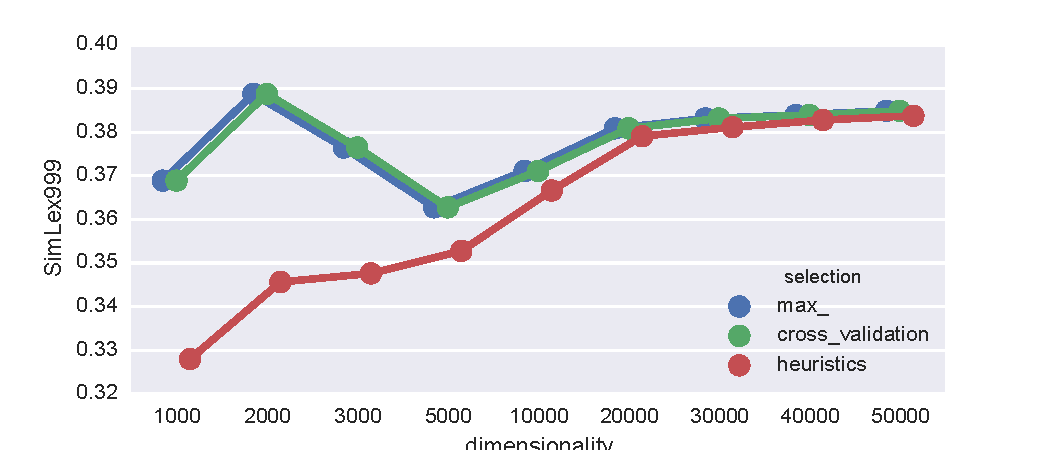
\includegraphics[width=0.5\textwidth]{supplement/figures/SimLex999-results}
  \caption{SimLex-999 results.}
  \label{fig:SimLex999-results}
\end{wrapfigure}

%%% Local Variables:
%%% mode: latex
%%% TeX-master: "../thesis"
%%% End:


\subsubsection{Max selection}
\label{sec:max-selection-simlex}

Figure~\ref{fig:SimLex999-results} illustrates the results based on the best model selection and Table~\ref{tab:parameters} shows the results together with picked parameters. Note that maximum selection is identical with cross-validation: they pick the same models.

In general model performance increases as the dimensionality increases. However, the best result of 0.389 is achieved with a 2000 dimensional space, this could be an example of overfitting. Model performance becomes changes for dimensions grater than 20000.

For spaces with dimensionality less than 5000 \texttt{freq} 1 and inner product yield best results. Otherwise, cosine with \logNSCPMI/, smoothing $\alpha=0.75$ and shifting $k=0.7$ gives the best results.

\begin{table}
  \centering

  \begin{tabular}{rrlllrl}
\toprule
 dimensionality &  SimLex999 &  freq &  discr &     cds &  neg &     similarity \\
\midrule
           1\,000 &      0.369 &     1 &   spmi &       1 &  0.2 &  inner\_product \\
           2\,000 &      0.389 &     1 &  scpmi &  global &  0.7 &  inner\_product \\
           3\,000 &      0.376 &     1 &   spmi &    0.75 &  0.2 &  inner\_product \\
           5\,000 &      0.363 &  logn &  scpmi &  global &  1.0 &            cos \\
          10\,000 &      0.371 &  logn &  scpmi &       1 &  0.7 &            cos \\
          20\,000 &      0.381 &  logn &  scpmi &    0.75 &  0.7 &            cos \\
          30\,000 &      0.383 &  logn &  scpmi &    0.75 &  0.7 &            cos \\
          40\,000 &      0.384 &  logn &  scpmi &    0.75 &  0.7 &            cos \\
          50\,000 &      0.385 &  logn &  scpmi &    0.75 &  0.7 &            cos \\
\bottomrule
\end{tabular}


  \caption{SimLex-999 Max selection.}
  \label{tab:Simlex999-max-selection}
\end{table}


\subsubsection{Heuristics}
\label{sec:heuristics-simlex}

\begin{wraptable}[8]{O}{0.5\textwidth}
  \vspace{-1em}
  \centering

  \begin{tabular}{lr}
\toprule
      parameter &  partial $R^2$ \\
\midrule
     similarity &       0.38 \\
           freq &       0.27 \\
            neg &       0.24 \\
 dimensionality &       0.08 \\
          discr &       0.08 \\
            cds &       0.06 \\
\bottomrule
\end{tabular}


  \caption{SimLex-999 feature ablation}
  \label{tab:SimLex999-ablation}
\end{wraptable}


% \begin{figure}

  \centering

  \begin{subfigure}[t]{0.49\textwidth}
    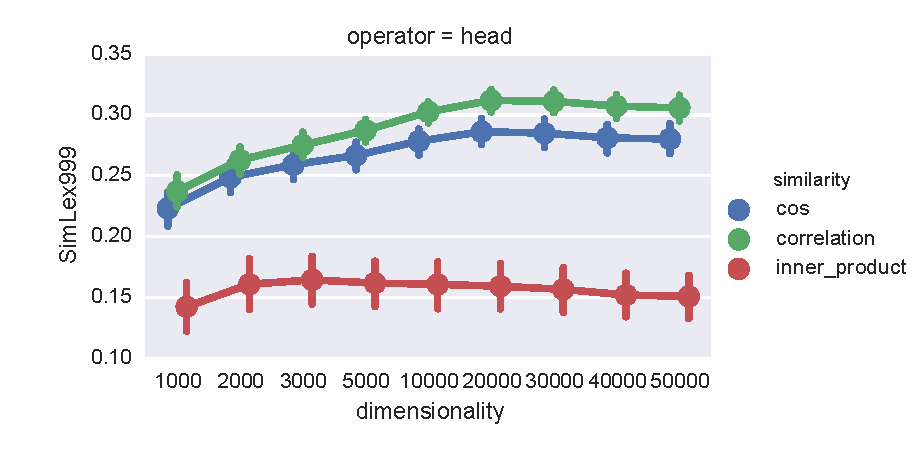
\includegraphics[width=\textwidth]{supplement/figures/SimLex999-interaction-similarity}
    \caption{similarity}
    \label{fig:SimLex999-interaction-similarity}
  \end{subfigure}
  \begin{subfigure}[t]{0.49\textwidth}
    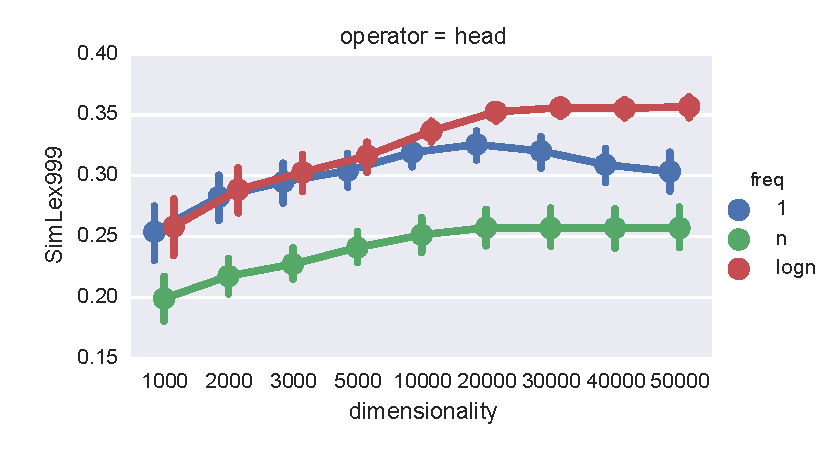
\includegraphics[width=\textwidth]{supplement/figures/SimLex999-interaction-freq}
    \caption{\texttt{freq}}
    \label{fig:SimLex999-interaction-freq}
  \end{subfigure}

  \begin{subfigure}[t]{0.49\textwidth}
    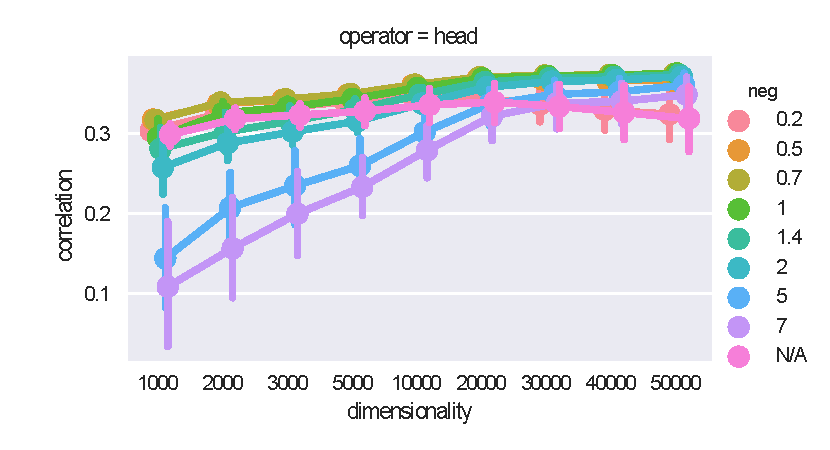
\includegraphics[width=\textwidth]{supplement/figures/SimLex999-interaction-neg}
    \caption{\texttt{neg}}
    \label{fig:SimLex999-interaction-neg}
  \end{subfigure}
  \begin{subfigure}[t]{0.49\textwidth}
    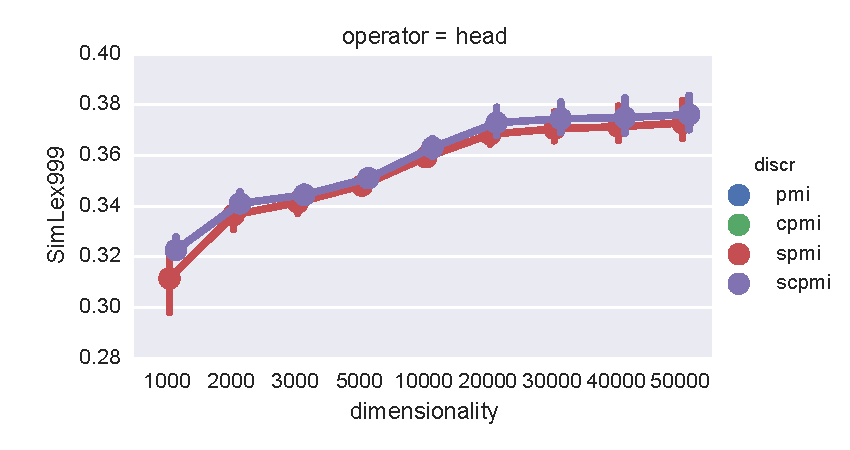
\includegraphics[width=\textwidth]{supplement/figures/SimLex999-interaction-discr}
    \caption{\texttt{discr}}
    \label{fig:SimLex999-interaction-discr}
  \end{subfigure}

  \begin{subfigure}[t]{0.49\textwidth}
    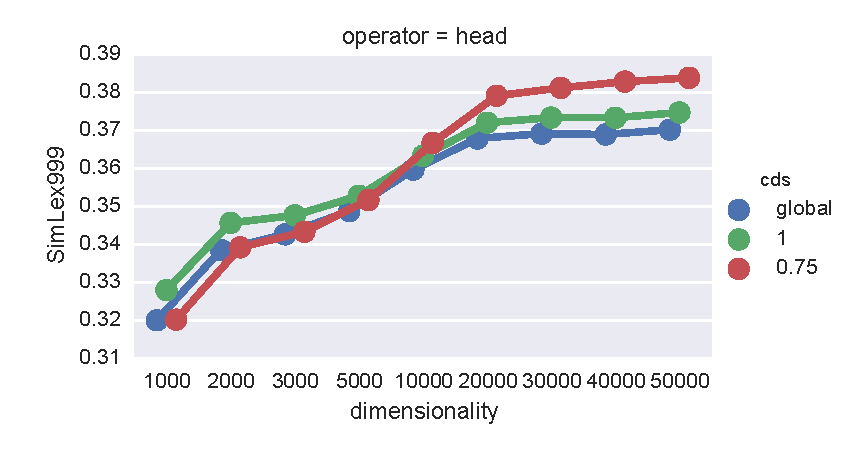
\includegraphics[width=\textwidth]{supplement/figures/SimLex999-interaction-cds}
    \caption{\texttt{cds}}
    \label{fig:SimLex999-interaction-cds}
  \end{subfigure}

  \caption{SimLex-999 parameter interaction. Parameters are shown in the order of their influence.}
  \label{fig:SimLex999-interaction}
\end{figure}

%%% Local Variables:
%%% mode: latex
%%% TeX-master: "../thesis"
%%% End:


The linear model achieves an adjusted $R^2$ of 0.867, indicating that the model is able to predict model performance based on parameter selection quite well. Table~\ref{tab:SimLex999-ablation} shows partial $R^2$ scores for parameters. The most influential parameters in decreasing order are similarity, \texttt{freq} and \texttt{neg}.

% \begin{wrapfigure}{O}{0.5\textwidth}
\begin{figure}
  % \vspace{-30pt}
  \centering

  \begin{subfigure}[t]{0.49\textwidth}
    \hspace{-20pt}
  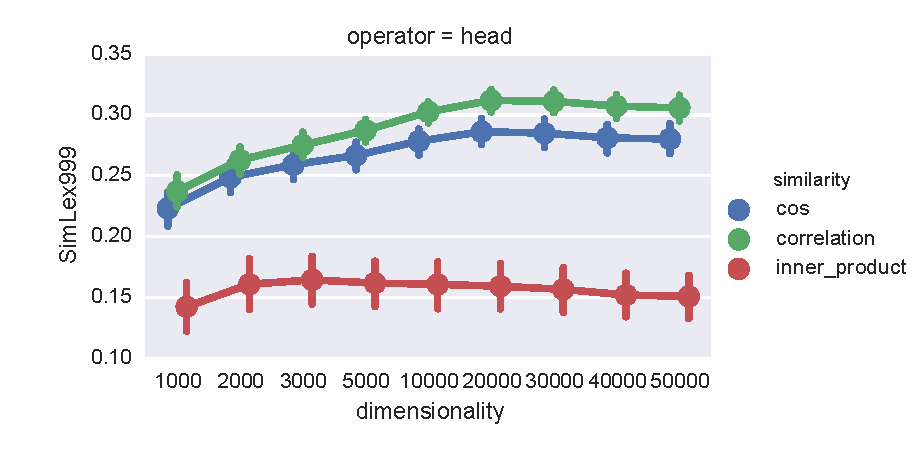
\includegraphics[width=1.1\textwidth]{supplement/figures/SimLex999-interaction-similarity}

  \caption{Similarity measure}
  \label{fig:SimLex999-similarity}

  \end{subfigure}
  \begin{subfigure}[t]{0.49\textwidth}

  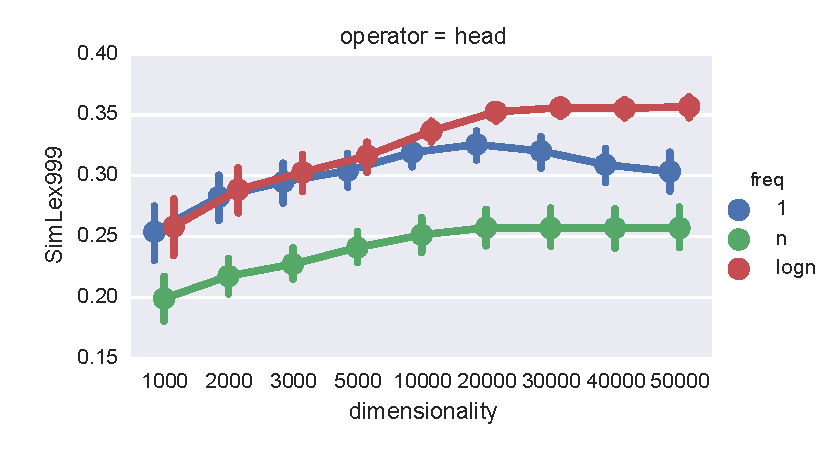
\includegraphics[width=\textwidth]{supplement/figures/SimLex999-interaction-freq}

  \caption{\texttt{freq}}
  \label{fig:SimLex999-freq}

  \end{subfigure}


  \begin{subfigure}[t]{0.49\textwidth}
  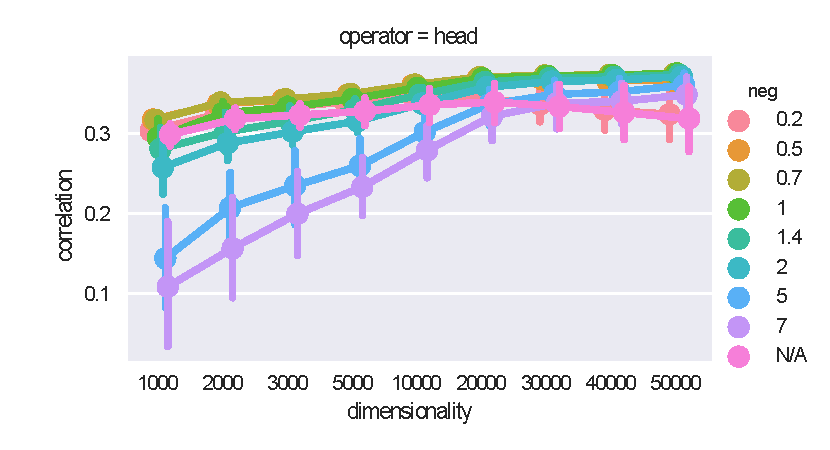
\includegraphics[width=\textwidth]{supplement/figures/SimLex999-interaction-neg}

  \caption{\texttt{neg}}
  \label{fig:SimLex999-neg}
  \end{subfigure}
  \begin{subfigure}[t]{0.49\textwidth}
  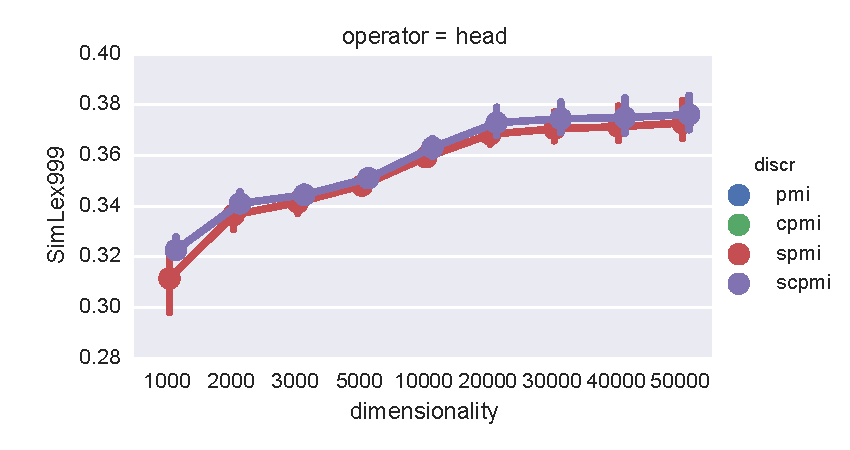
\includegraphics[width=\textwidth]{supplement/figures/SimLex999-interaction-discr}

  \caption{\texttt{discr}}
  \label{fig:SimLex999-discr}
  \end{subfigure}
  
  \caption[SimLex-999 influence of the similarity measure, \texttt{freq}, \texttt{neg} and \texttt{discr}]{SimLex-999 influence of the similarity measure, \texttt{freq}, \texttt{neg} and \texttt{discr}. Error bars indicate the 95\% confidence interval over the group of results.}
\end{figure}

Figure~\ref{fig:SimLex999-similarity} shows the average performance of similarity measures. Correlation outperforms all other measures for all dimensions and peaks at the dimensionality of 20000.

\begin{figure}[h]
% \begin{wrapfigure}{O}{0.5\textwidth}
  % \vspace{-30pt}
  \centering

  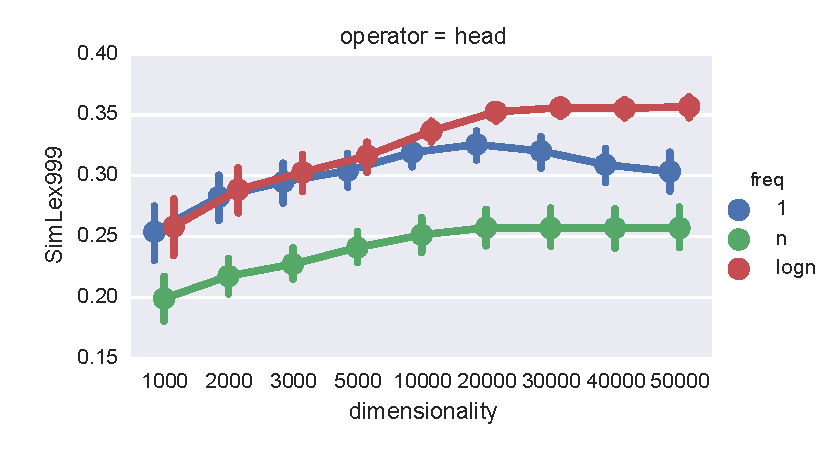
\includegraphics[width=0.5\textwidth]{supplement/figures/SimLex999-interaction-freq}

  \caption{SimLex-999 influence of \texttt{freq}.}
  \label{fig:SimLex999-freq}
\end{figure}

The influence of \texttt{freq}, the second parameter, is shown on Figure~\ref{fig:SimLex999-freq}. $\log n$ frequency outperforms other choices for all dimensions. After 20000 dimensions $\log n$'s performance stabilises.

\begin{figure}[b]
% \begin{wrapfigure}{O}{0.5\textwidth}
  % \vspace{-30pt}
  \centering

  \begin{subfigure}[t]{0.49\textwidth}
  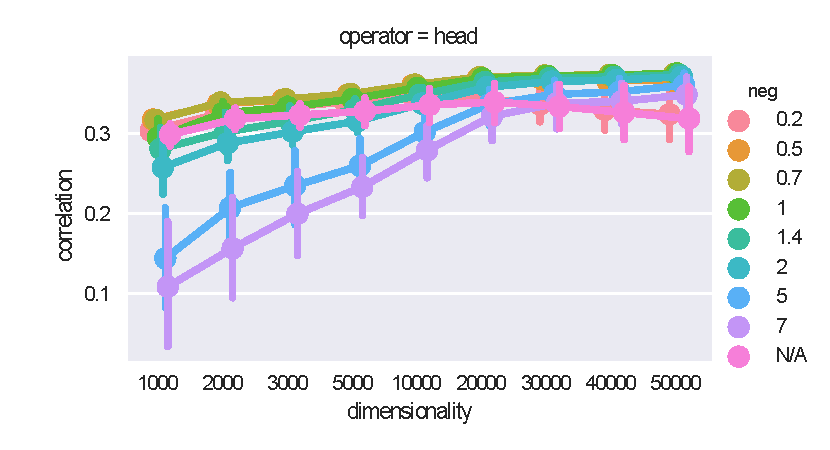
\includegraphics[width=\textwidth]{supplement/figures/SimLex999-interaction-neg}

  \caption{\texttt{neg}}
  \label{fig:SimLex999-neg}
  \end{subfigure}
  \begin{subfigure}[t]{0.49\textwidth}
  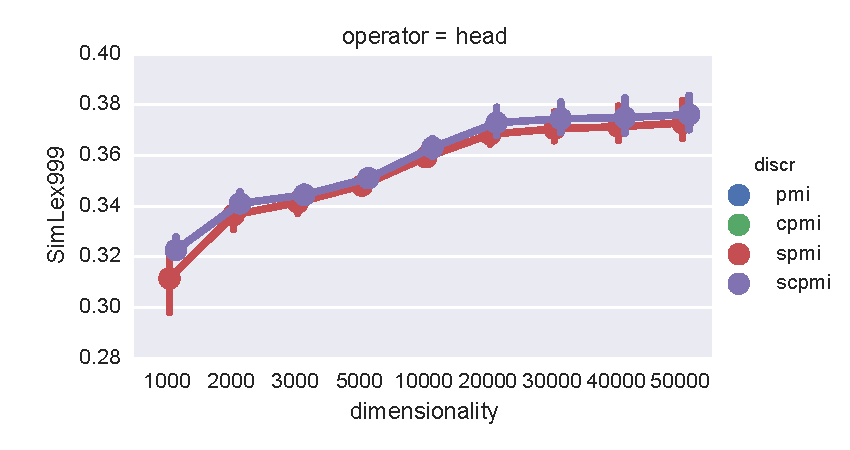
\includegraphics[width=\textwidth]{supplement/figures/SimLex999-interaction-discr}

  \caption{\texttt{discr}}
  \label{fig:SimLex999-discr}
  \end{subfigure}

  \caption{SimLex-999.}
\end{figure}

The third parameter \texttt{neg} of 0.7 shows the best performance (Figure~\ref{fig:SimLex999-neg}). However, there is little difference between models with dimensionality grater than 20000, apart from the models that do not perform shifting, whose performance peaks at 20000 dimensions.

\begin{figure}[h]
% \begin{wrapfigure}{O}{0.5\textwidth}
  % \vspace{-30pt}
  \centering

  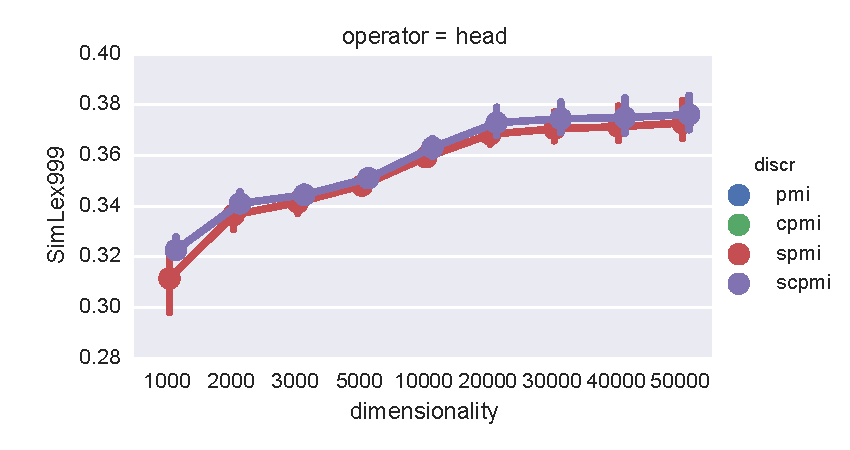
\includegraphics[width=0.5\textwidth]{supplement/figures/SimLex999-interaction-discr}

  \caption{SimLex-999 influence of \texttt{discr}. PMI and CPMI are not shown because at the step before models with shifting were chosen.}
  \label{fig:SimLex999-discr}
\end{figure}

There is little difference between SPMI and SCPMI performance with a little advantage to SCPMI (Figure~\ref{fig:SimLex999-discr}).

% \begin{figure}[h]
\begin{wrapfigure}[5]{O}{0.5\textwidth}
  \vspace{-30pt}
  \centering

  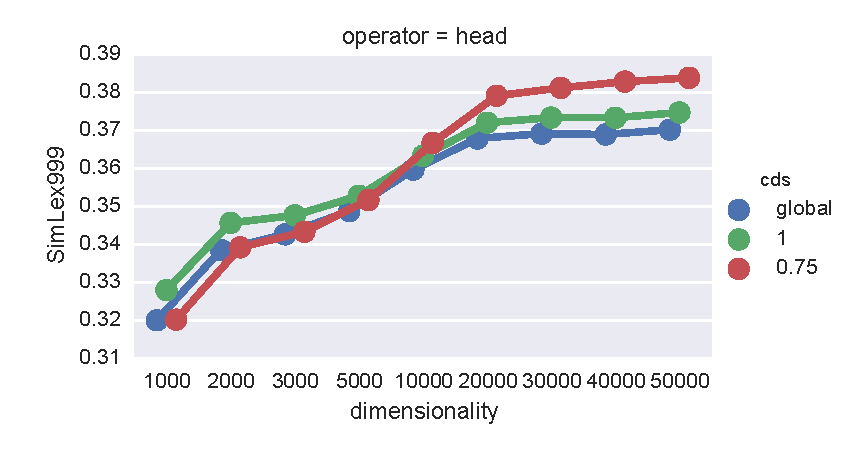
\includegraphics[width=0.5\textwidth]{supplement/figures/SimLex999-interaction-cds}
  \caption{SimLex-999 influence of \texttt{cds}.}
  \label{fig:SimLex999-cds}
\end{wrapfigure}

Finally, models benefit from context distribution smoothing, spaces with less than 10000 dimensions produce the best results with $\alpha = 1$, for spaces with higher dimensionality $\alpha = 0.75$ is the most advantageous (Figure~\ref{fig:SimLex999-cds}).

\todo[noline]{Contrast or compare results with \cite{milajevs:2016:SRW1}}

\paragraph{Difference with "Max" selection}

\begin{table}
  \centering

  \begin{tabular}{rrlllll}
\toprule
 dimensionality &  SimLex999 &  freq &  discr &   cds &  neg &   similarity \\
\midrule
           1\,000 &      0.328 &  logn &  scpmi &     1 &  0.7 &  correlation \\
           2\,000 &      0.346 &  logn &  scpmi &     1 &  0.7 &  correlation \\
           3\,000 &      0.348 &  logn &  scpmi &     1 &  0.7 &  correlation \\
           5\,000 &      0.353 &  logn &  scpmi &     1 &  0.7 &  correlation \\
          10\,000 &      0.367 &  logn &  scpmi &  0.75 &  0.7 &  correlation \\
          20\,000 &      0.379 &  logn &  scpmi &  0.75 &  0.7 &  correlation \\
          30\,000 &      0.381 &  logn &  scpmi &  0.75 &  0.7 &  correlation \\
          40\,000 &      0.383 &  logn &  scpmi &  0.75 &  0.7 &  correlation \\
          \textbf{50\,000} &      \textbf{0.384} &  \textbf{logn} &  \textbf{scpmi} &  \textbf{0.75} &  \textbf{0.7} &  \textbf{correlation} \\
\bottomrule
\end{tabular}


  \caption{SimLex-999 selection based on heuristics. The highest value is 0.384.
  The values that are grater than 0.361 are indistinguishable from the highest score.}
  \label{tab:Simlex999-heuristics-selection}
\end{table}


As expected manual parameter selection is more stable. Both selection models agree on parameters for highly dimensional spaces ($D \geq 2000$), with an exception of similarity: Max selection prefers cosine, while manual prefers correlation based similarity measure. Because of this, manual selection does not pick the best result of the 2000 dimensional model, but at the 50000 dimensions  a model selected manually scores 0.001 lower: 0.384 versus 0.385 as also seen on Figure~\ref{fig:SimLex999-results}.

The average relative difference between Max selection and heuristics is 0.039.

\subsection{MEN}
\label{sec:men}

\subsubsection{Max selection}
\label{sec:max-selection-men}

\begin{figure}
  \centering

    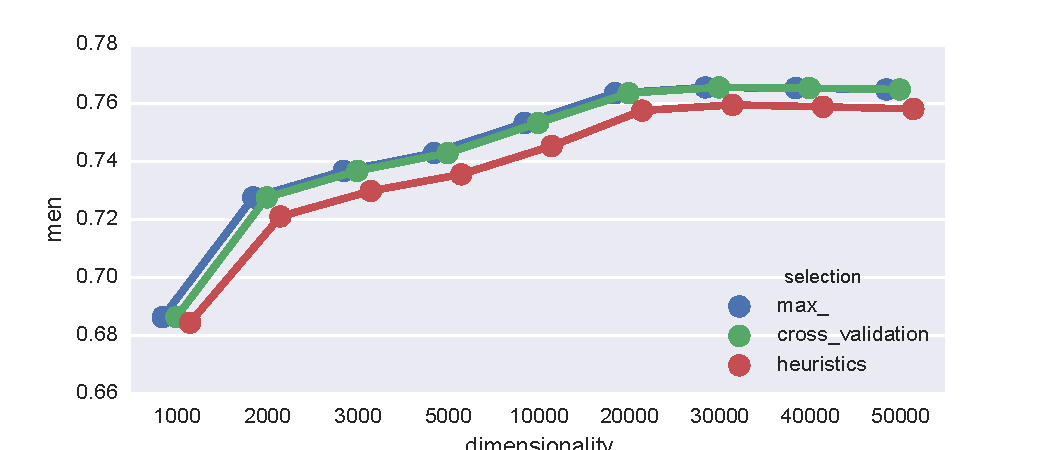
\includegraphics[width=0.5\textwidth]{supplement/figures/men-results}
  \caption{MEN results.}
  \label{fig:men-results}
\end{figure}

%%% Local Variables:
%%% mode: latex
%%% TeX-master: "../thesis"
%%% End:


Figure~\ref{fig:SimLex999-results} shows the selection results. Again, cross-validation results are identical with Max selection. Table~\ref{tab:men-max-selection} shows the results together with the selected models.

\begin{table}[b]
  \centering

  \begin{tabular}{rrlllrl}
\toprule
 dimensionality &    men &  freq &  discr &     cds &  neg &   similarity \\
\midrule
           1\,000 &  0.686 &     1 &  scpmi &  global &  1.4 &  correlation \\
           2\,000 &  0.728 &  logn &  scpmi &       1 &  0.7 &          cos \\
           3\,000 &  0.737 &  logn &  scpmi &       1 &  0.7 &          cos \\
           5\,000 &  0.743 &  logn &  scpmi &    0.75 &  0.7 &          cos \\
          10\,000 &  0.753 &  logn &  scpmi &    0.75 &  1.0 &  correlation \\
          20\,000 &  0.763 &  logn &  scpmi &    0.75 &  1.0 &  correlation \\
          \textbf{30\,000} &  \textbf{0.765} &  \textbf{logn} &  \textbf{scpmi} &    \textbf{0.75} &  \textbf{1.0} &  \textbf{correlation} \\
          \textbf{40\,000} &  \textbf{0.765} &  \textbf{logn} &  \textbf{scpmi} &    \textbf{0.75} &  \textbf{1.0} &  \textbf{correlation} \\
          \textbf{50\,000} &  \textbf{0.765} &  \textbf{logn} &  \textbf{scpmi} &    \textbf{0.75} &  \textbf{1.0} &  \textbf{correlation} \\
\bottomrule
\end{tabular}


  \caption{MEN Max selection}
  \label{tab:men-max-selection}
\end{table}


\subsubsection{Heuristics}
\label{sec:heuristics-men}


\subsection{Universal parameter selection for lexical datasets}
\label{sec:Universal-lexical-param-selection}

% SimLex --> Men
% Men --> SimLex
% Universal, normalized!

% Idea: find common parameters and take average over one for which there is not agreement. Normalize the result and repeat the heuristics selection?

\section{Similarity of sentences}
\label{sec:sentential}

\subsection{KS14}
\label{sec:ks14}


% \clearpage
% \KOMAoptions{paper=A3}
% % \addtolength{\textwidth}{1.35\textwidth}
% \recalctypearea

\newgeometry{margin=1.5cm}

\begin{landscape}
\thispagestyle{empty} %% Remove header and footer.

\begin{figure}
  \centering

  \begin{subfigure}[t]{0.49\textwidth}
    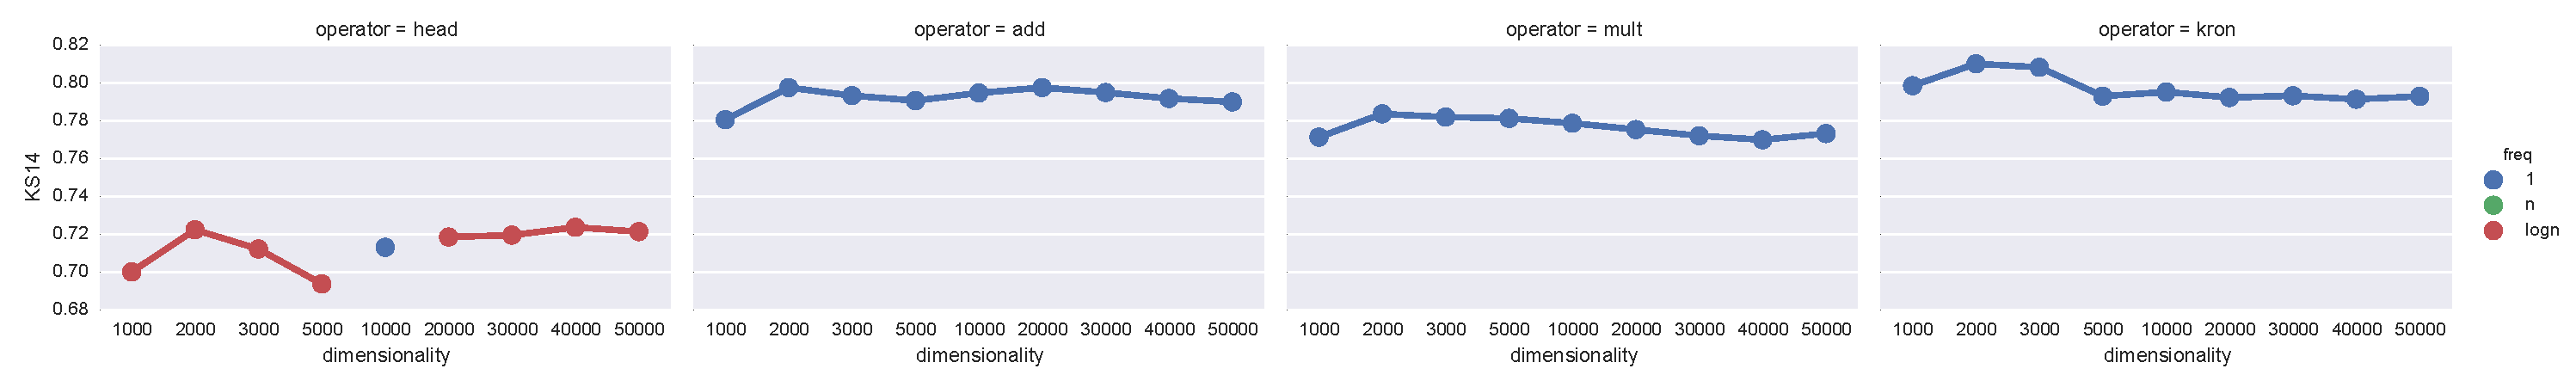
\includegraphics[width=\textwidth]{supplement/figures/KS14-max_-selection-freq}
    \caption{Max. Freq.}
    \label{fig:}
  \end{subfigure}
  \begin{subfigure}[t]{0.49\textwidth}
    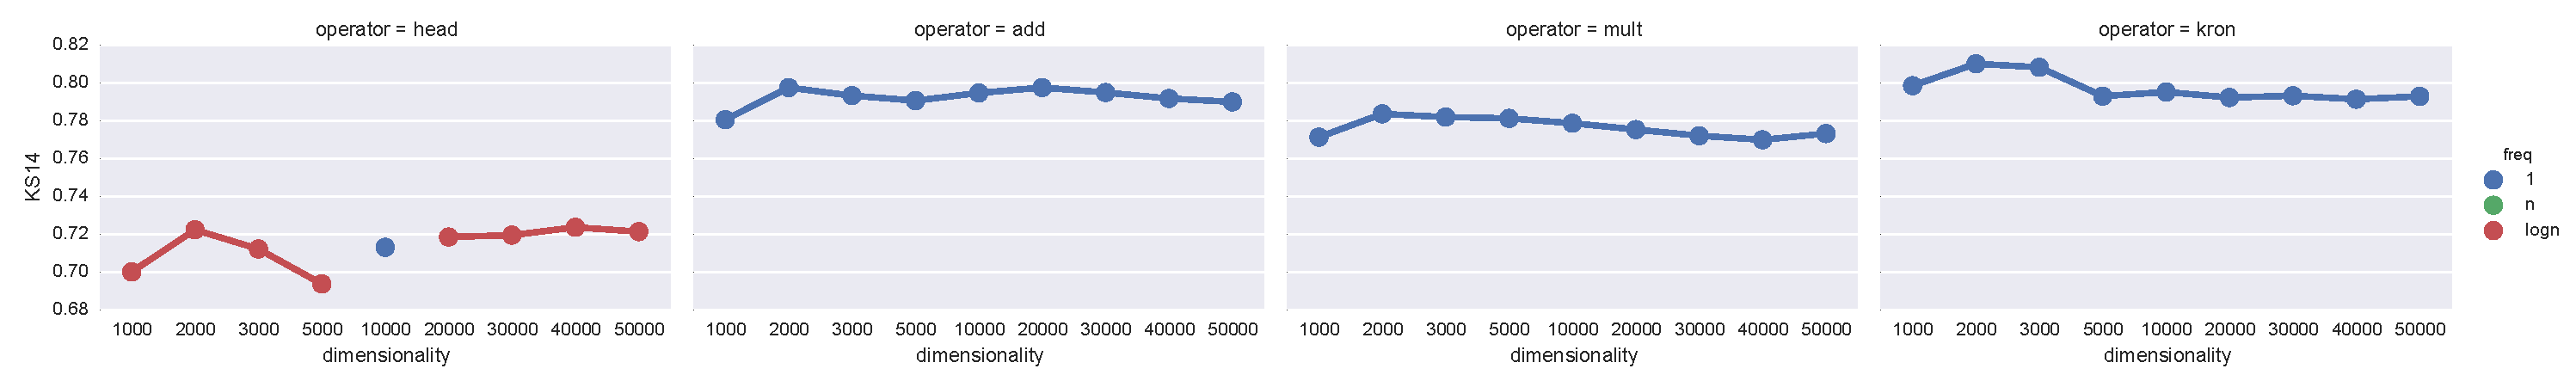
\includegraphics[width=\textwidth]{supplement/figures/KS14-cross_validation-selection-freq}
    \caption{CV. Freq.}
    \label{fig:}
  \end{subfigure}
  \begin{subfigure}[t]{0.49\textwidth}
    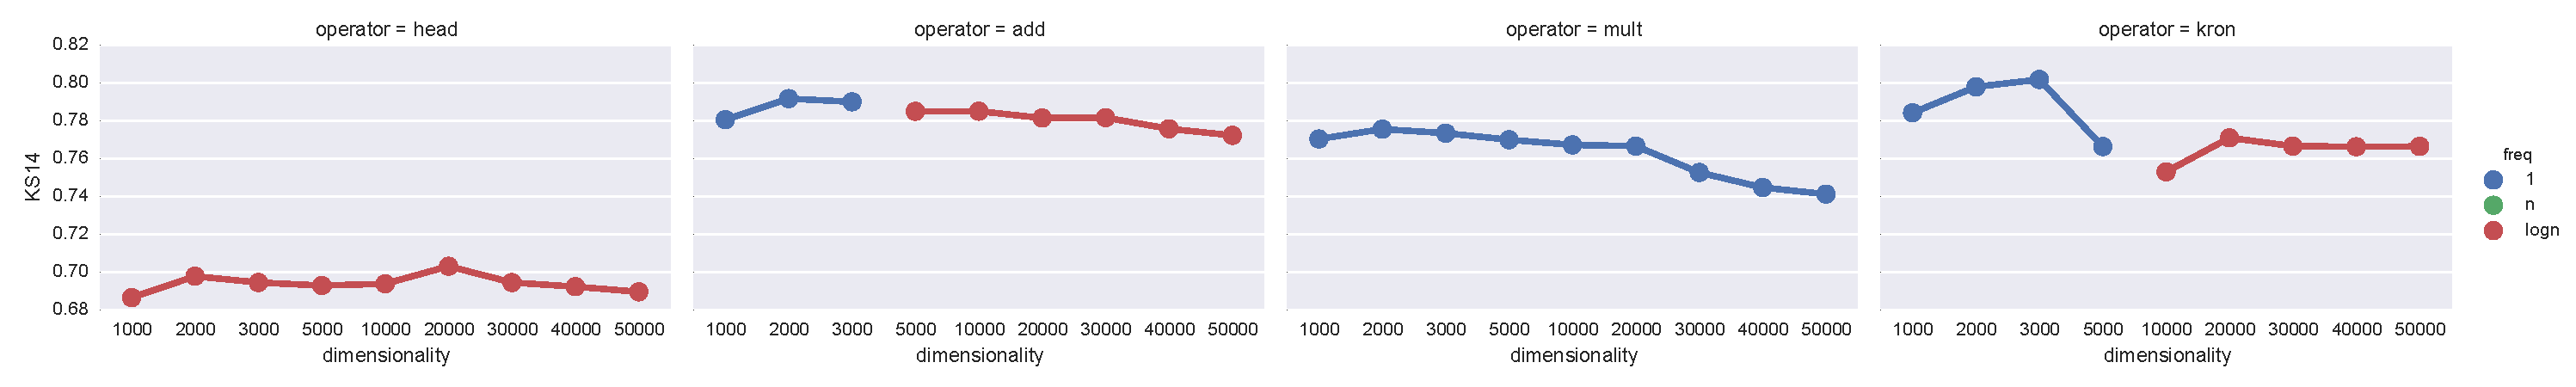
\includegraphics[width=\textwidth]{supplement/figures/KS14-heuristics-selection-freq}
    \caption{H. Freq.}
    \label{fig:}
  \end{subfigure}

  \begin{subfigure}[t]{0.49\textwidth}
    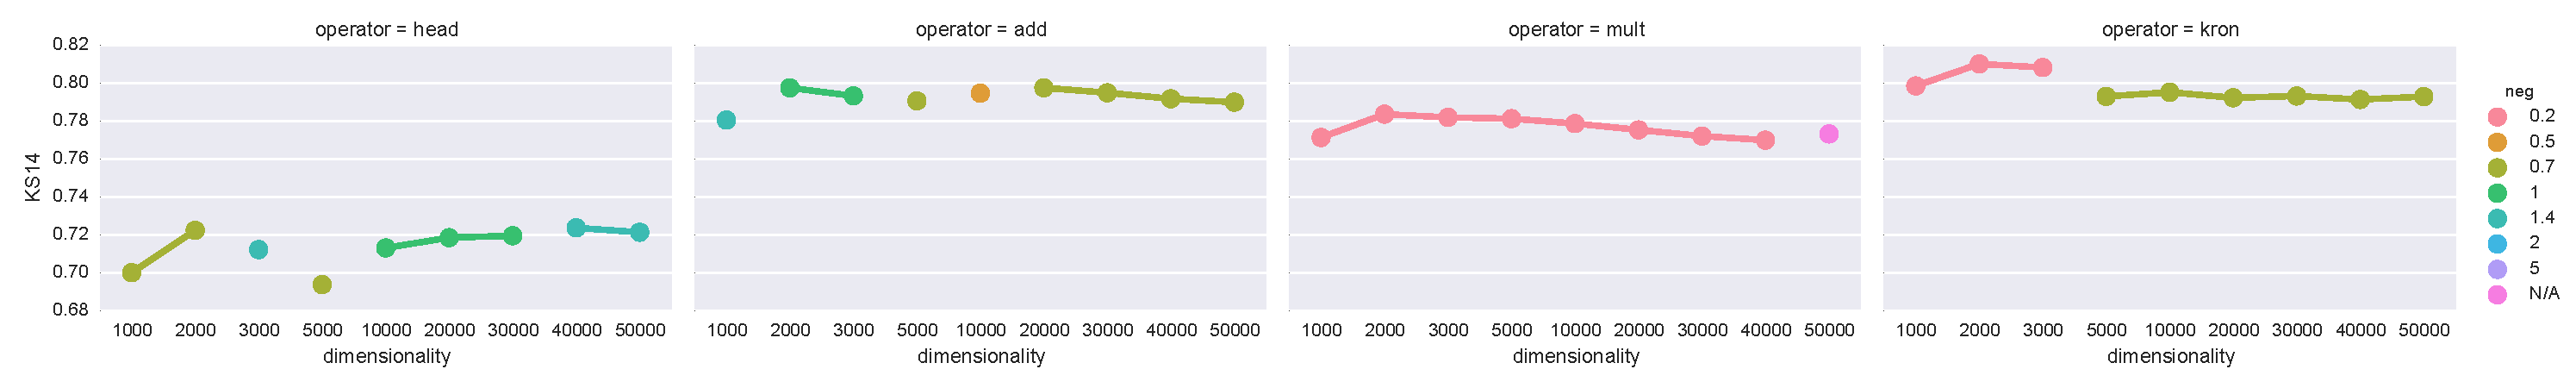
\includegraphics[width=\textwidth]{supplement/figures/KS14-max_-selection-neg}
    \caption{Max. Neg.}
    \label{fig:}
  \end{subfigure}
  \begin{subfigure}[t]{0.49\textwidth}
    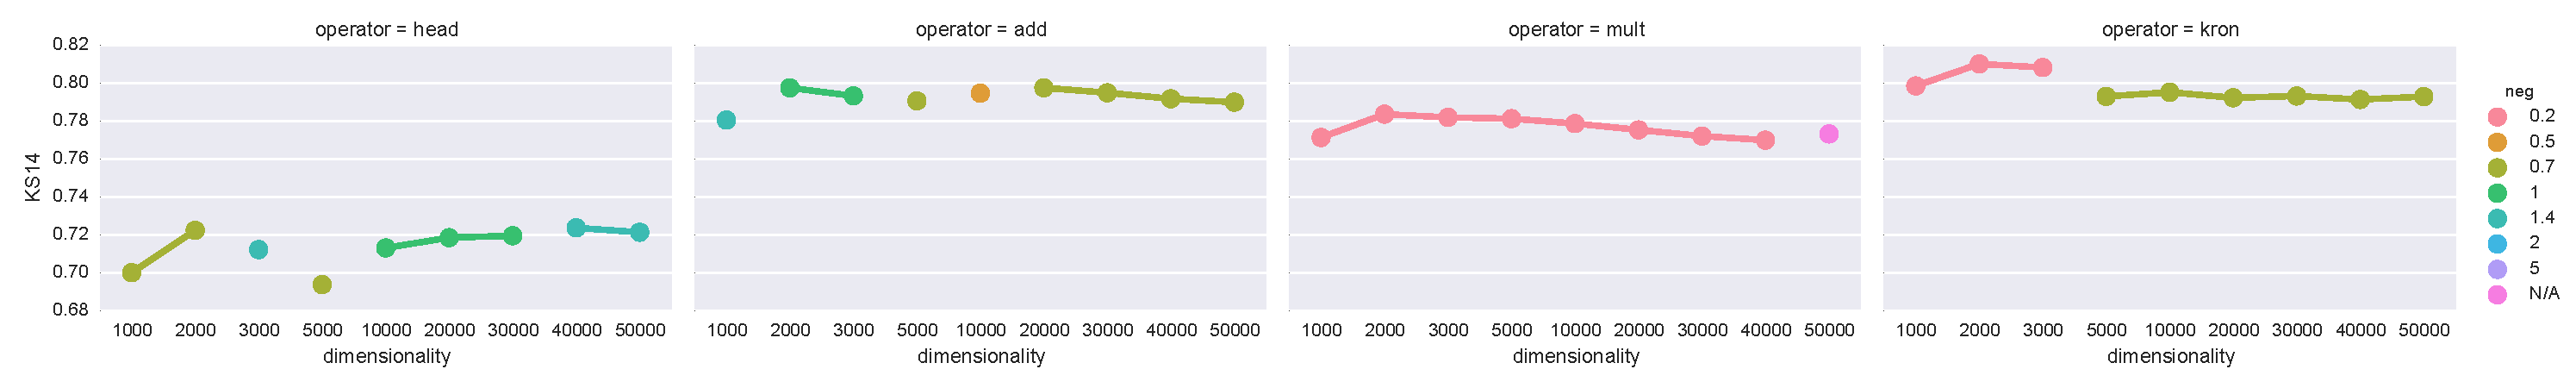
\includegraphics[width=\textwidth]{supplement/figures/KS14-cross_validation-selection-neg}
    \caption{CV. Neg.}
    \label{fig:}
  \end{subfigure}
  \begin{subfigure}[t]{0.49\textwidth}
    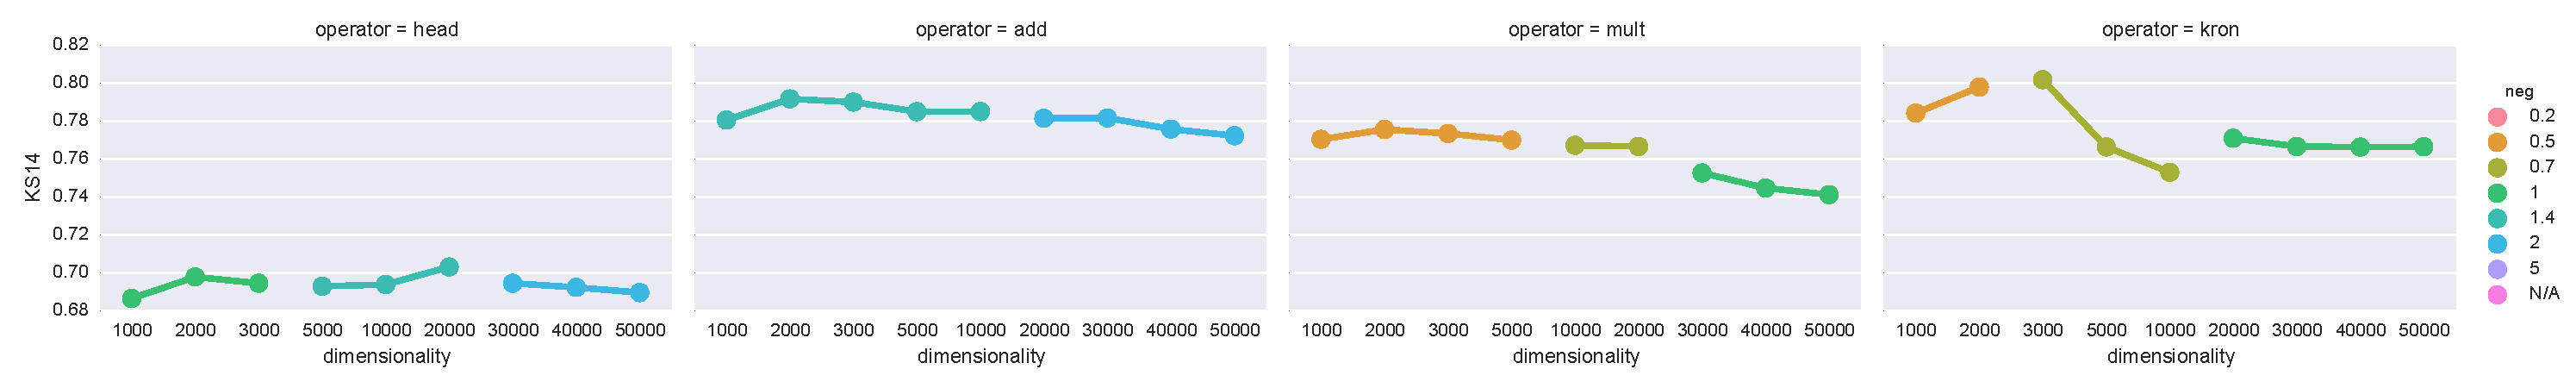
\includegraphics[width=\textwidth]{supplement/figures/KS14-heuristics-selection-neg}
    \caption{H. Neg.}
    \label{fig:}
  \end{subfigure}

  \begin{subfigure}[t]{0.49\textwidth}
    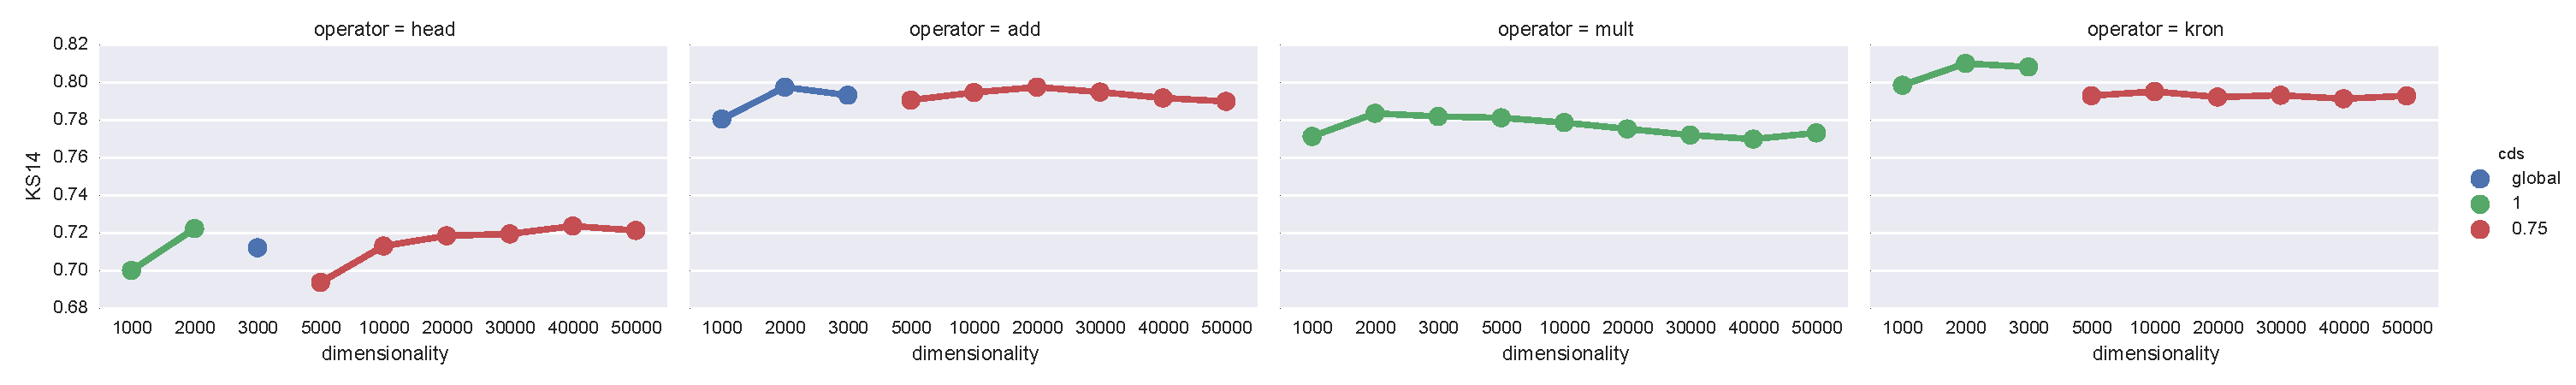
\includegraphics[width=\textwidth]{supplement/figures/KS14-max_-selection-cds}
    \caption{Max. CDS.}
    \label{fig:}
  \end{subfigure}
  \begin{subfigure}[t]{0.49\textwidth}
    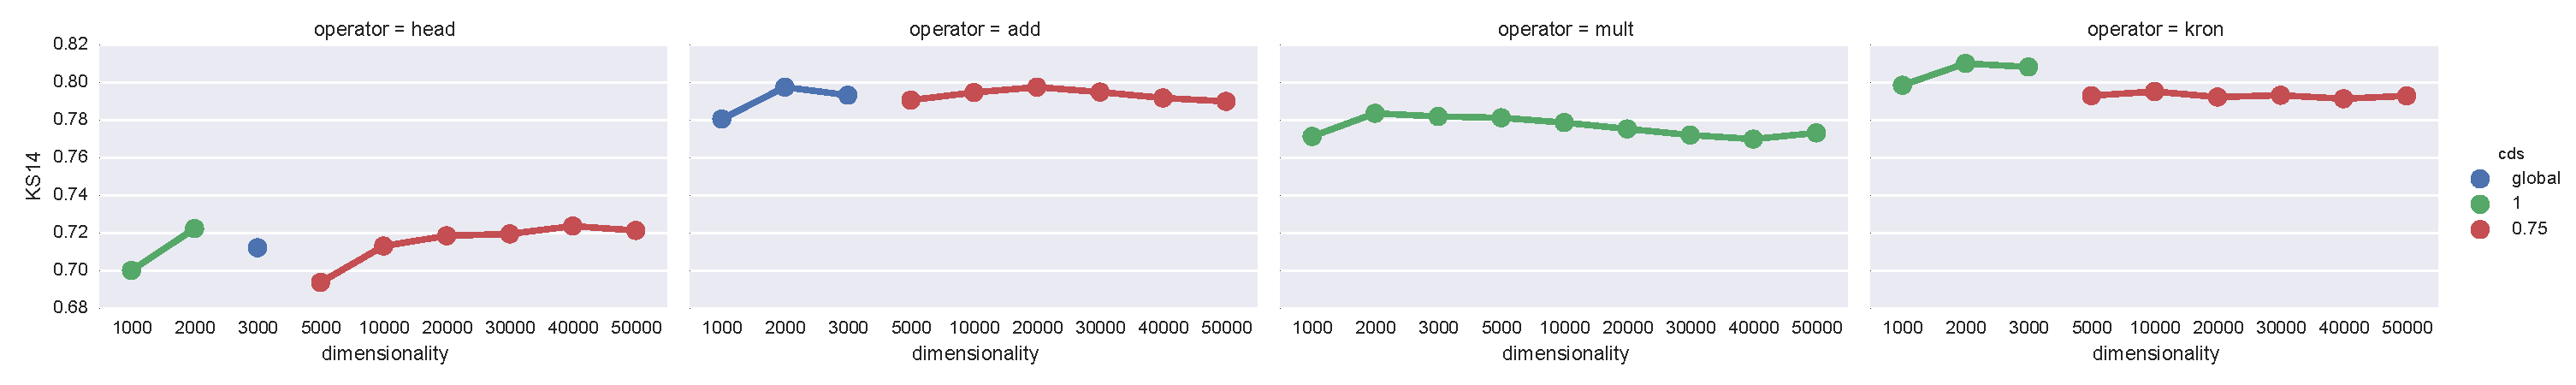
\includegraphics[width=\textwidth]{supplement/figures/KS14-cross_validation-selection-cds}
    \caption{CV. CDS.}
    \label{fig:}
  \end{subfigure}
  \begin{subfigure}[t]{0.49\textwidth}
    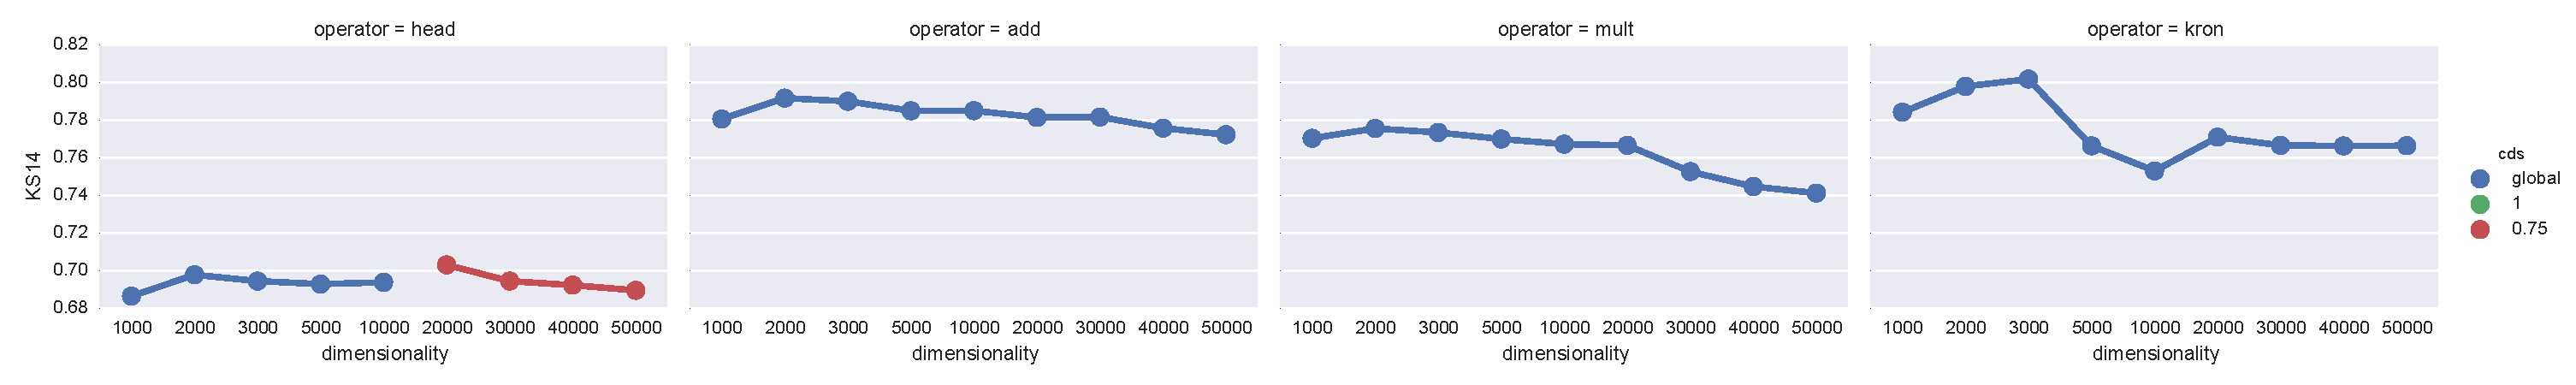
\includegraphics[width=\textwidth]{supplement/figures/KS14-heuristics-selection-cds}
    \caption{H. CDS.}
    \label{fig:}
  \end{subfigure}

  \begin{subfigure}[t]{0.49\textwidth}
    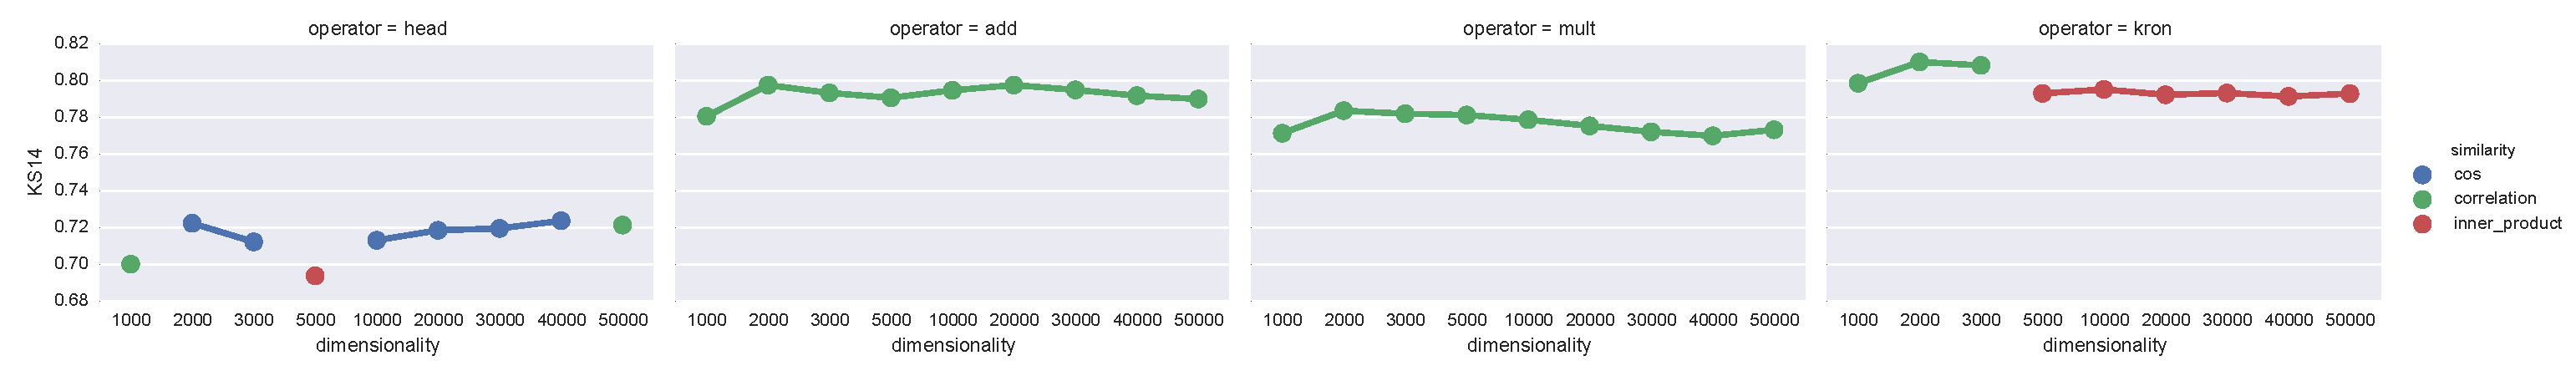
\includegraphics[width=\textwidth]{supplement/figures/KS14-max_-selection-similarity}
    \caption{Max. Sim.}
    \label{fig:}
  \end{subfigure}
  \begin{subfigure}[t]{0.49\textwidth}
    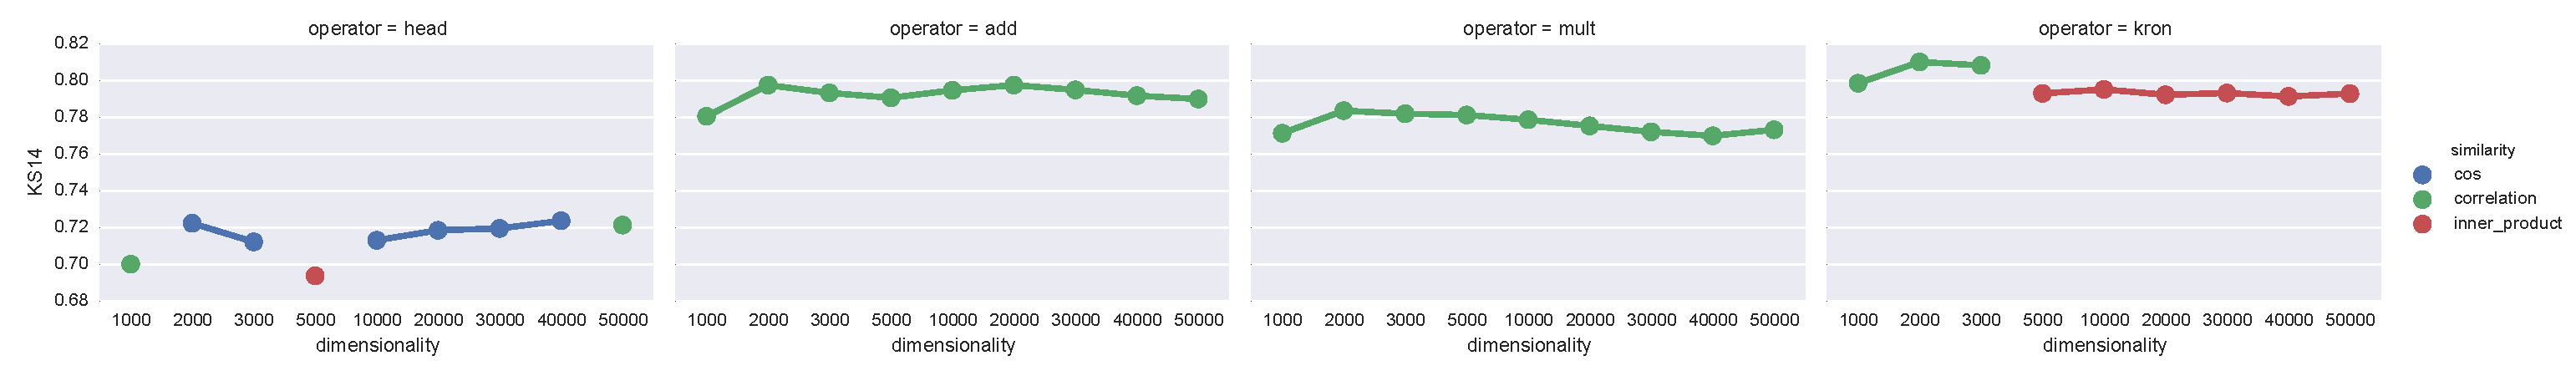
\includegraphics[width=\textwidth]{supplement/figures/KS14-cross_validation-selection-similarity}
    \caption{CV. Sim.}
    \label{fig:}
  \end{subfigure}
  \begin{subfigure}[t]{0.49\textwidth}
    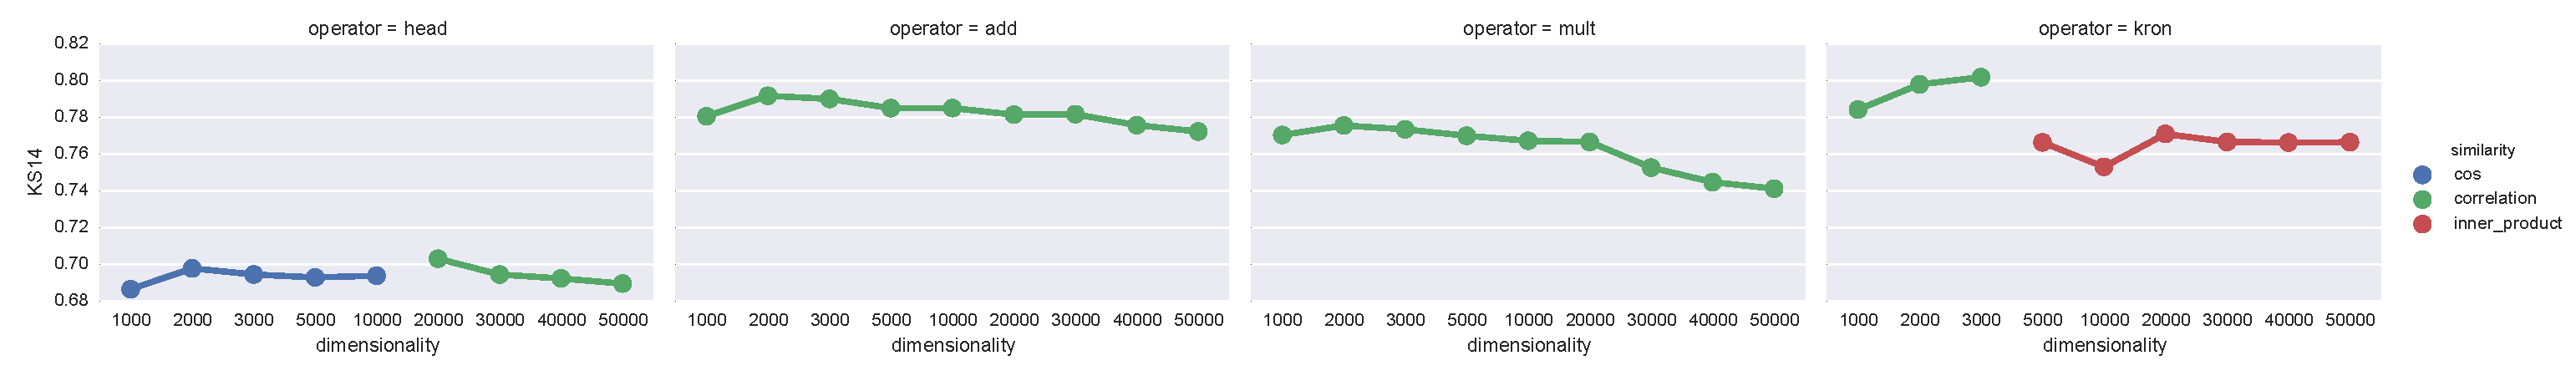
\includegraphics[width=\textwidth]{supplement/figures/KS14-heuristics-selection-similarity}
    \caption{H. Sim.}
    \label{fig:}
  \end{subfigure}

  \begin{subfigure}[t]{0.49\textwidth}
    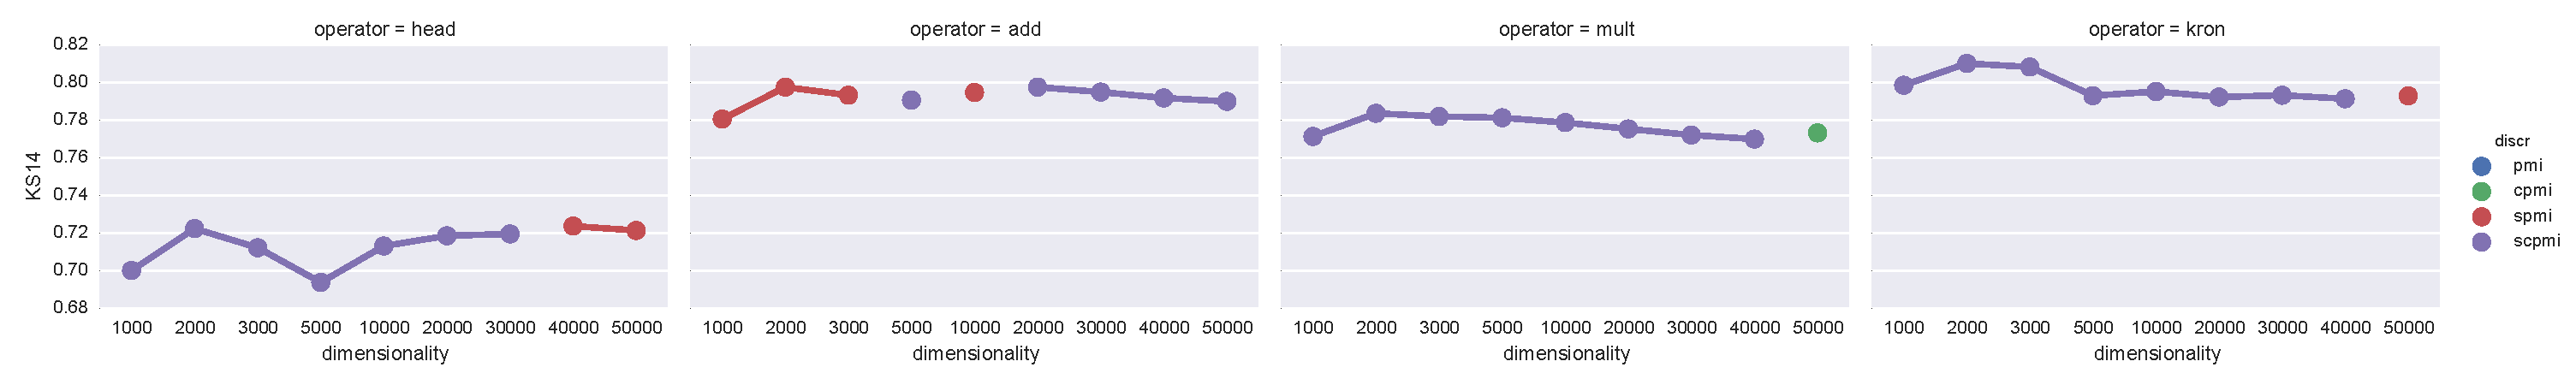
\includegraphics[width=\textwidth]{supplement/figures/KS14-max_-selection-discr}
    \caption{Max. Discr.}
    \label{fig:}
  \end{subfigure}
  \begin{subfigure}[t]{0.49\textwidth}
    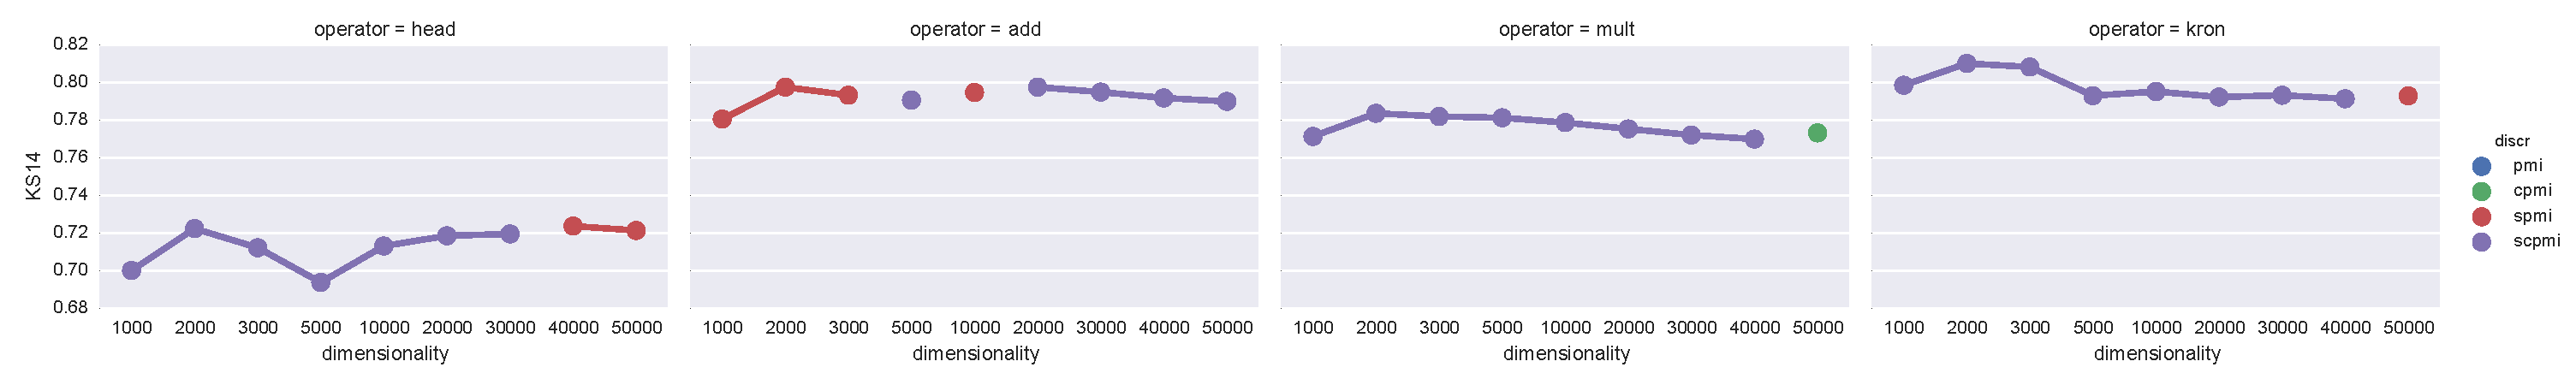
\includegraphics[width=\textwidth]{supplement/figures/KS14-cross_validation-selection-discr}
    \caption{CV. Discr.}
    \label{fig:}
  \end{subfigure}
  \begin{subfigure}[t]{0.49\textwidth}
    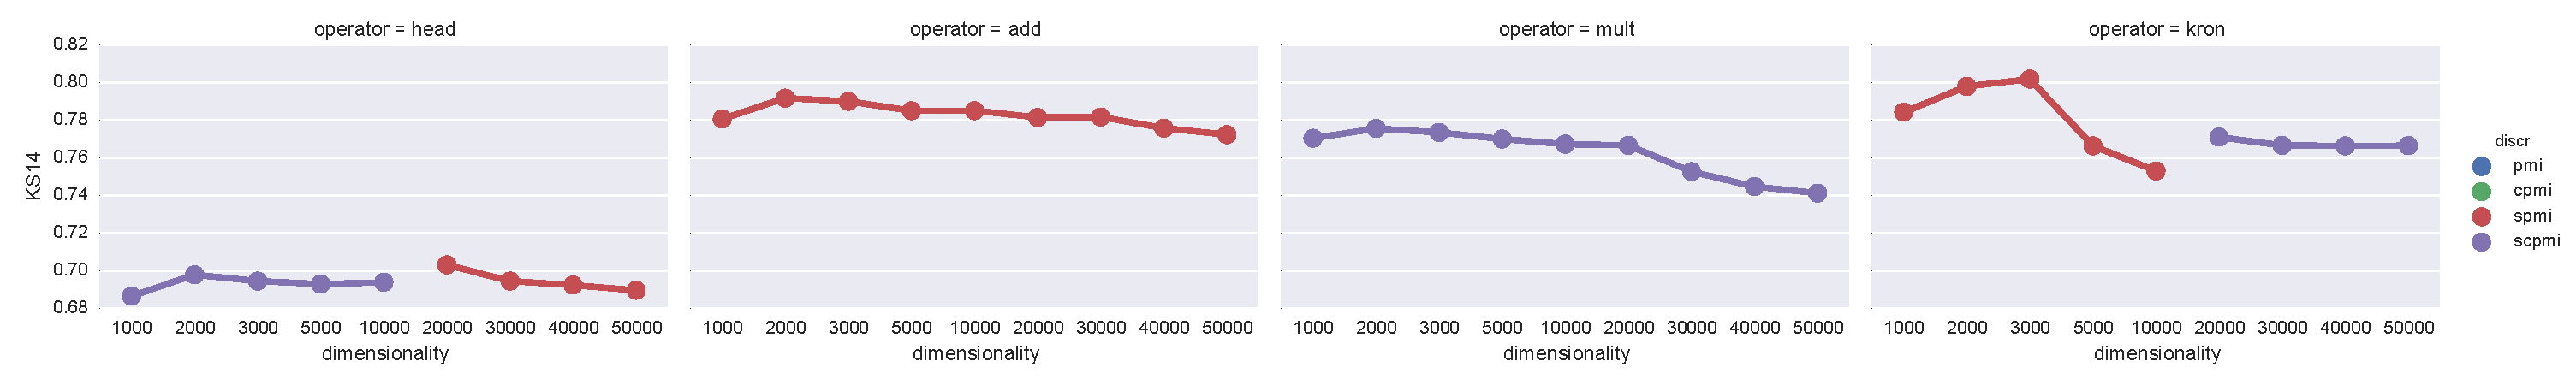
\includegraphics[width=\textwidth]{supplement/figures/KS14-heuristics-selection-discr}
    \caption{H. Discr.}
    \label{fig:}
  \end{subfigure}


  \caption{KS14 selection.}
  \label{fig:selection_ks14}
\end{figure}

\end{landscape}

\restoregeometry

% \clearpage
% \KOMAoptions{paper=A4,pagesize}
% \recalctypearea


\subsection{GS11}
\label{sec:gs11}

% \clearpage
% \KOMAoptions{paper=A3}
% % \addtolength{\textwidth}{1.35\textwidth}
% \recalctypearea

\newgeometry{margin=1.5cm}

\begin{landscape}
% \thispagestyle{empty} %% Remove header and footer.

\begin{figure}
  \centering

  \begin{subfigure}[t]{0.7\textwidth}
    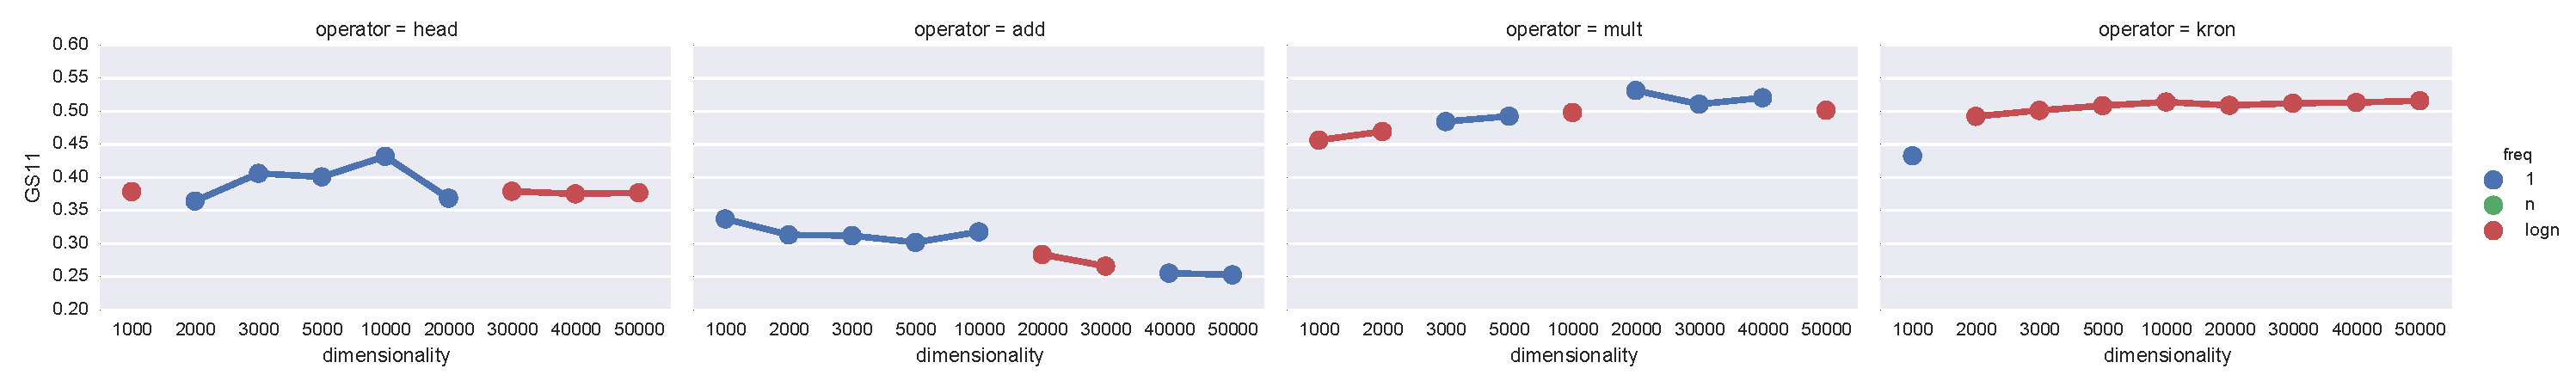
\includegraphics[width=\textwidth]{supplement/figures/GS11-max_-selection-freq}
    \caption{Max. Freq.}
    \label{fig:}
  \end{subfigure}
  % \begin{subfigure}[t]{0.7\textwidth}
  %   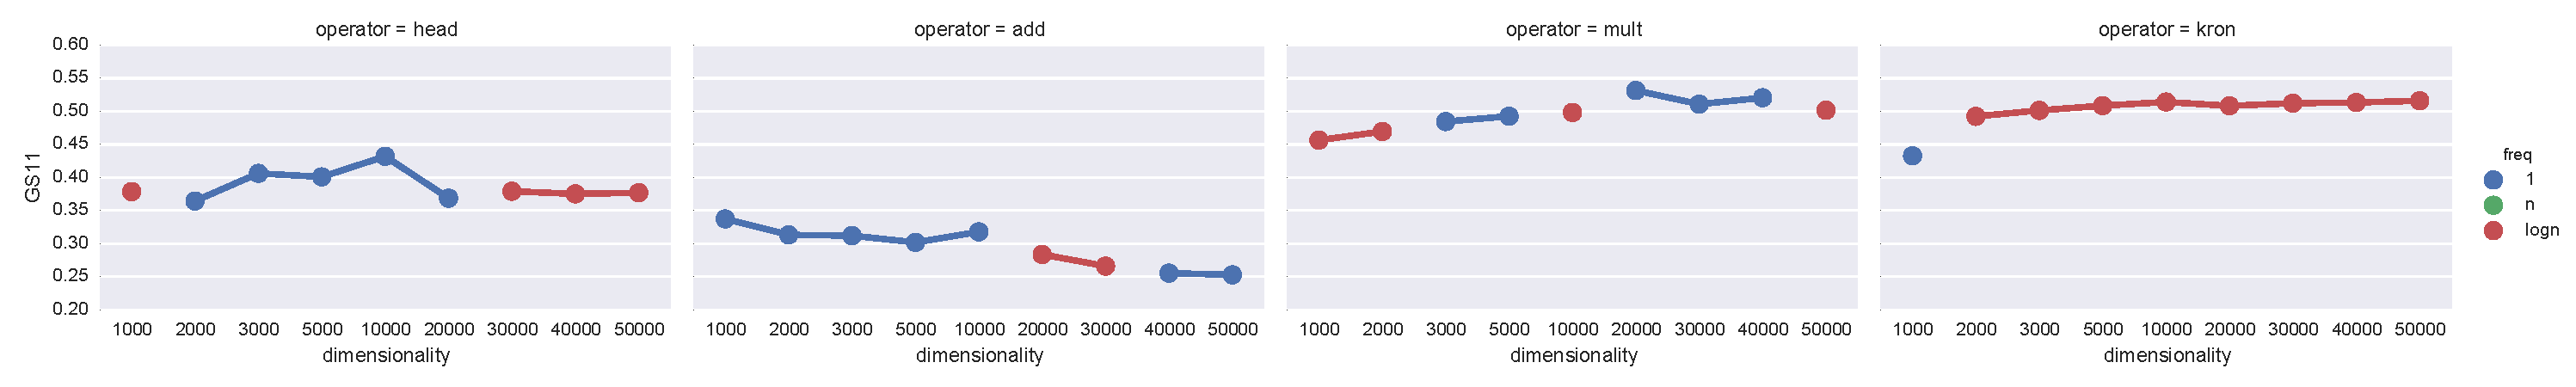
\includegraphics[width=\textwidth]{supplement/figures/GS11-cross_validation-selection-freq}
  %   \caption{CV. Freq.}
  %   \label{fig:}
  % \end{subfigure}
  \begin{subfigure}[t]{0.7\textwidth}
    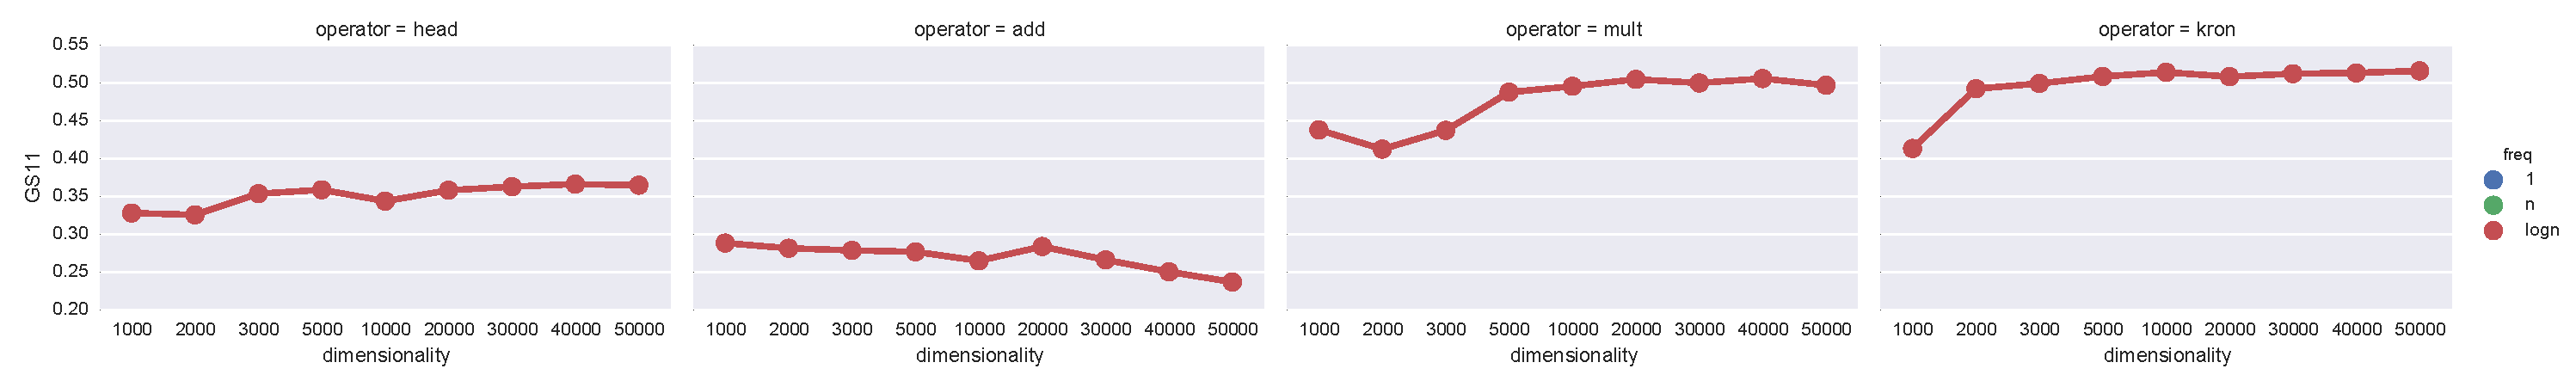
\includegraphics[width=\textwidth]{supplement/figures/GS11-heuristics-selection-freq}
    \caption{H. Freq.}
    \label{fig:}
  \end{subfigure}

  \begin{subfigure}[t]{0.7\textwidth}
    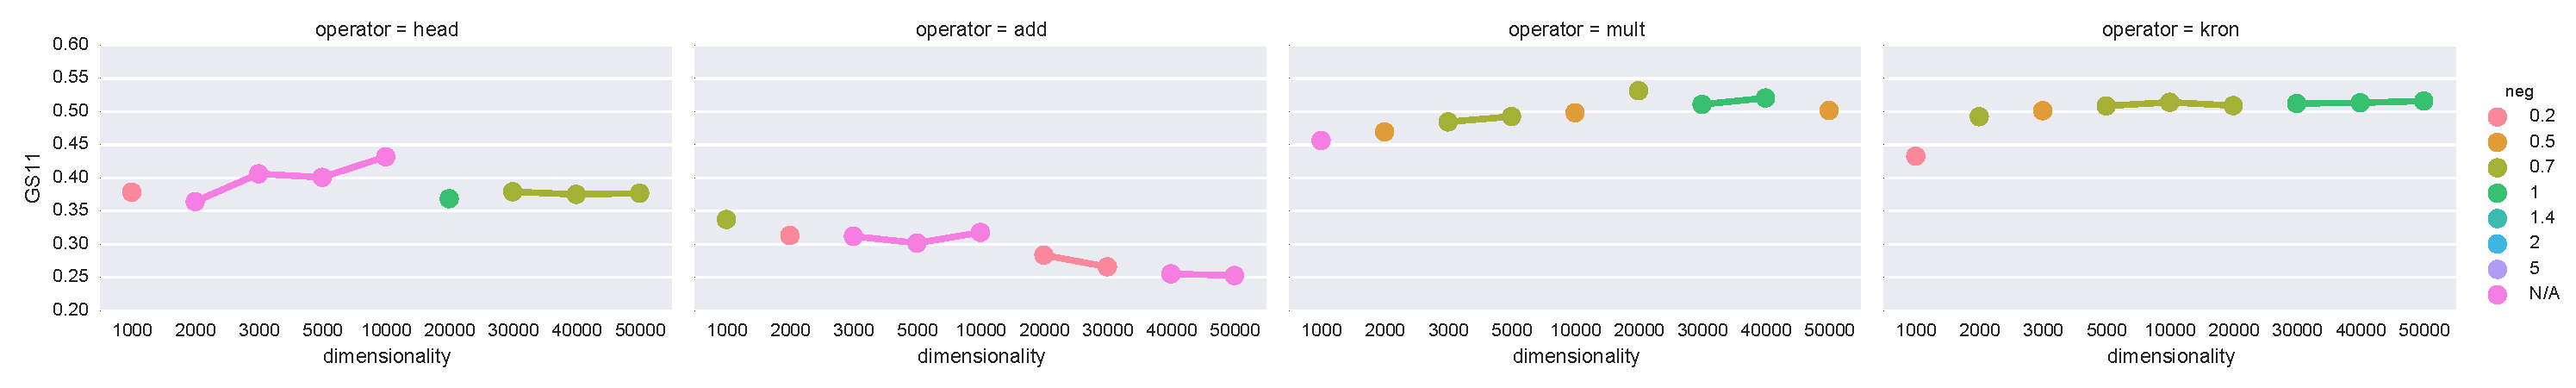
\includegraphics[width=\textwidth]{supplement/figures/GS11-max_-selection-neg}
    \caption{Max. Neg.}
    \label{fig:}
  \end{subfigure}
  % \begin{subfigure}[t]{0.7\textwidth}
  %   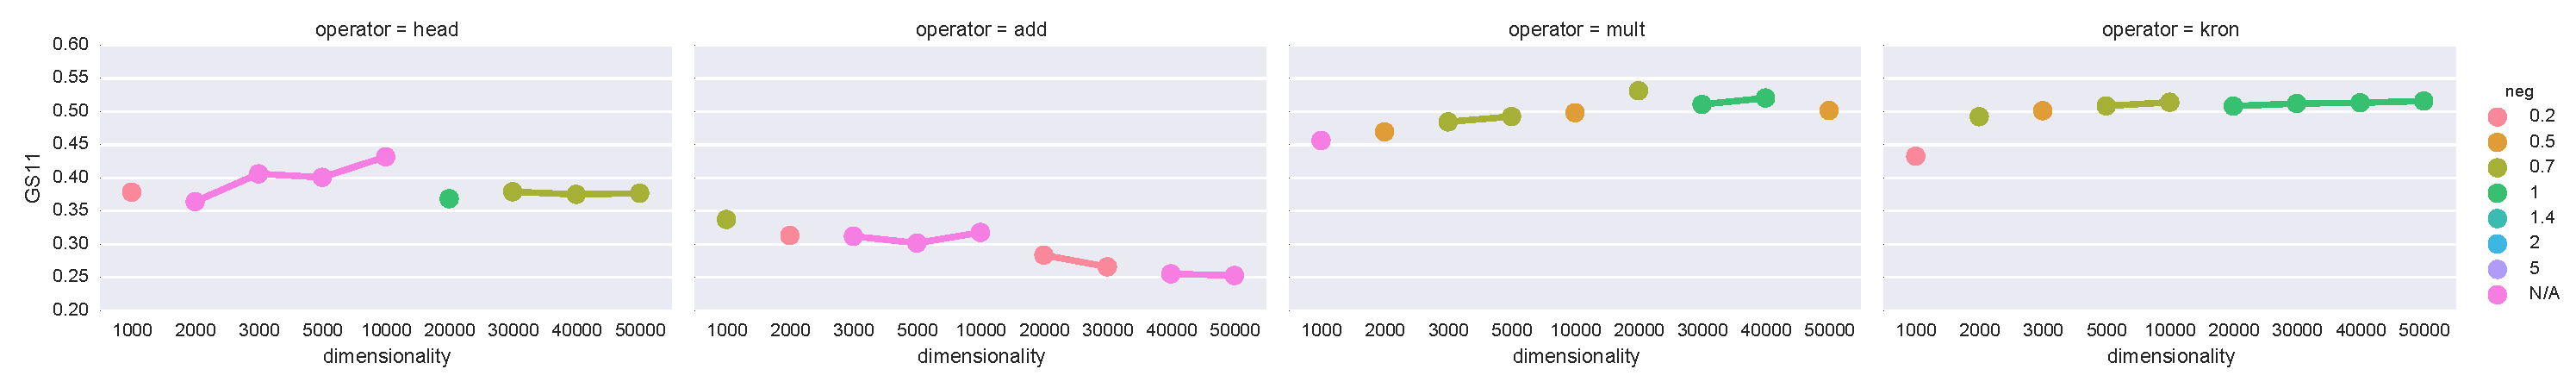
\includegraphics[width=\textwidth]{supplement/figures/GS11-cross_validation-selection-neg}
  %   \caption{CV. Neg.}
  %   \label{fig:}
  % \end{subfigure}
  \begin{subfigure}[t]{0.7\textwidth}
    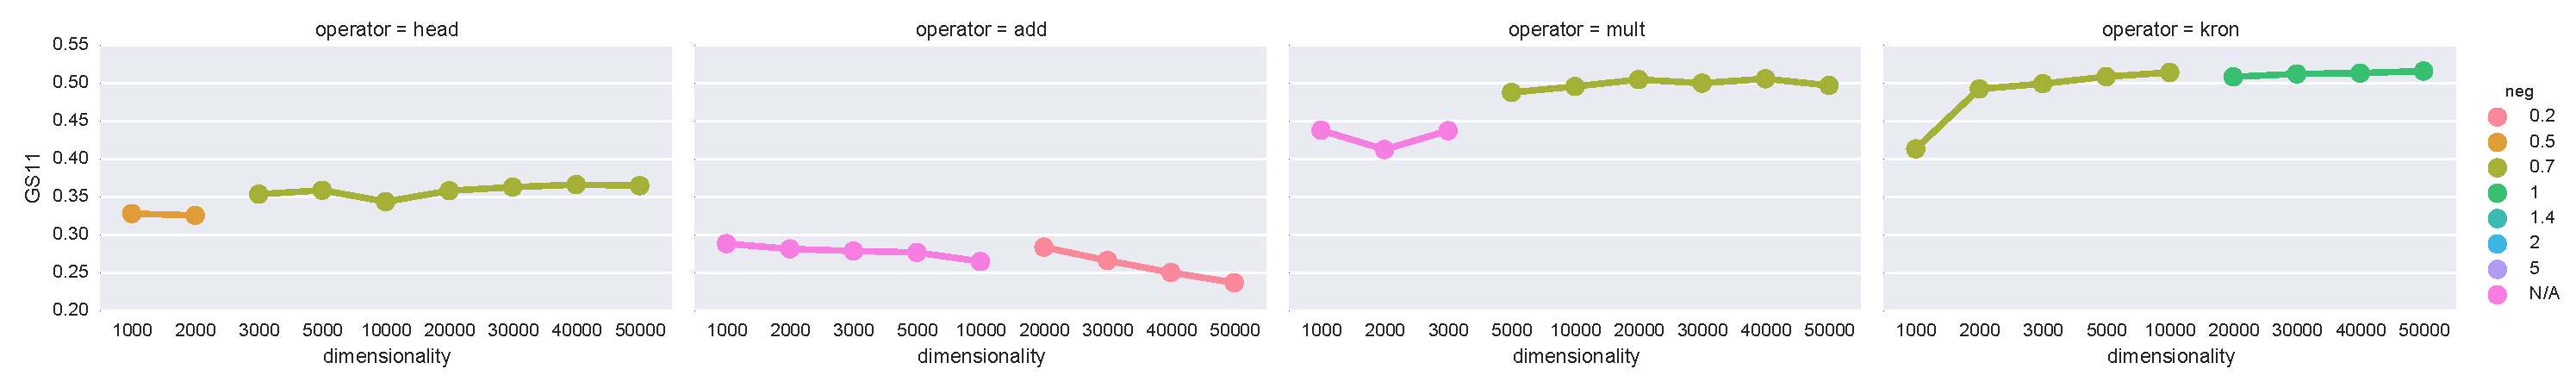
\includegraphics[width=\textwidth]{supplement/figures/GS11-heuristics-selection-neg}
    \caption{H. Neg.}
    \label{fig:}
  \end{subfigure}

  \begin{subfigure}[t]{0.7\textwidth}
    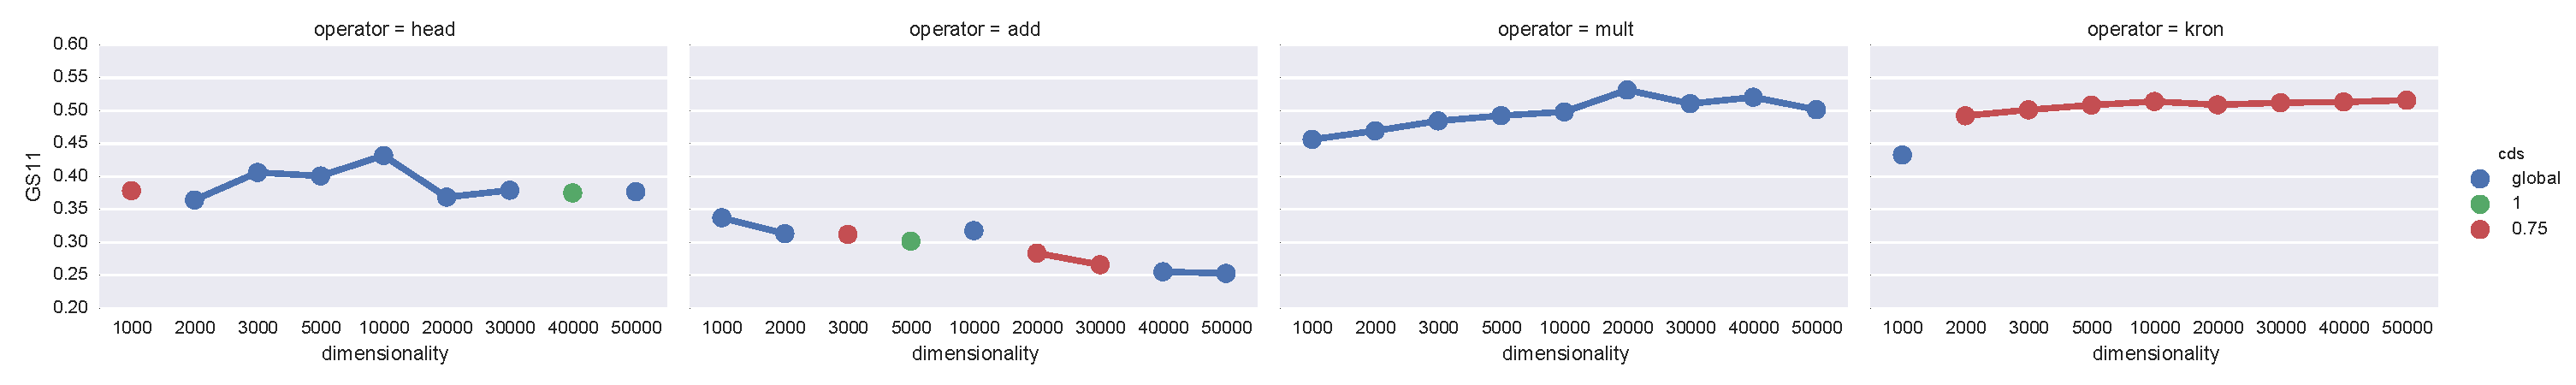
\includegraphics[width=\textwidth]{supplement/figures/GS11-max_-selection-cds}
    \caption{Max. CDS.}
    \label{fig:}
  \end{subfigure}
  % \begin{subfigure}[t]{0.7\textwidth}
  %   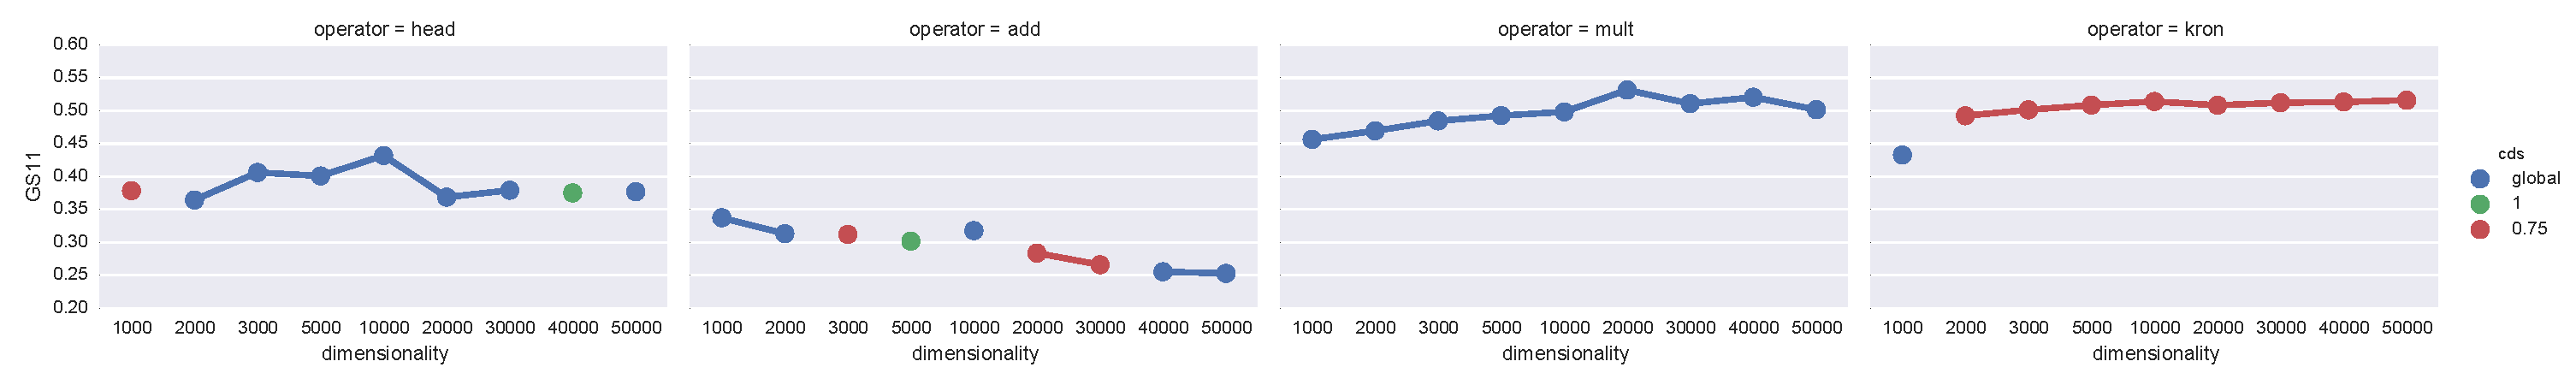
\includegraphics[width=\textwidth]{supplement/figures/GS11-cross_validation-selection-cds}
  %   \caption{CV. CDS.}
  %   \label{fig:}
  % \end{subfigure}
  \begin{subfigure}[t]{0.7\textwidth}
    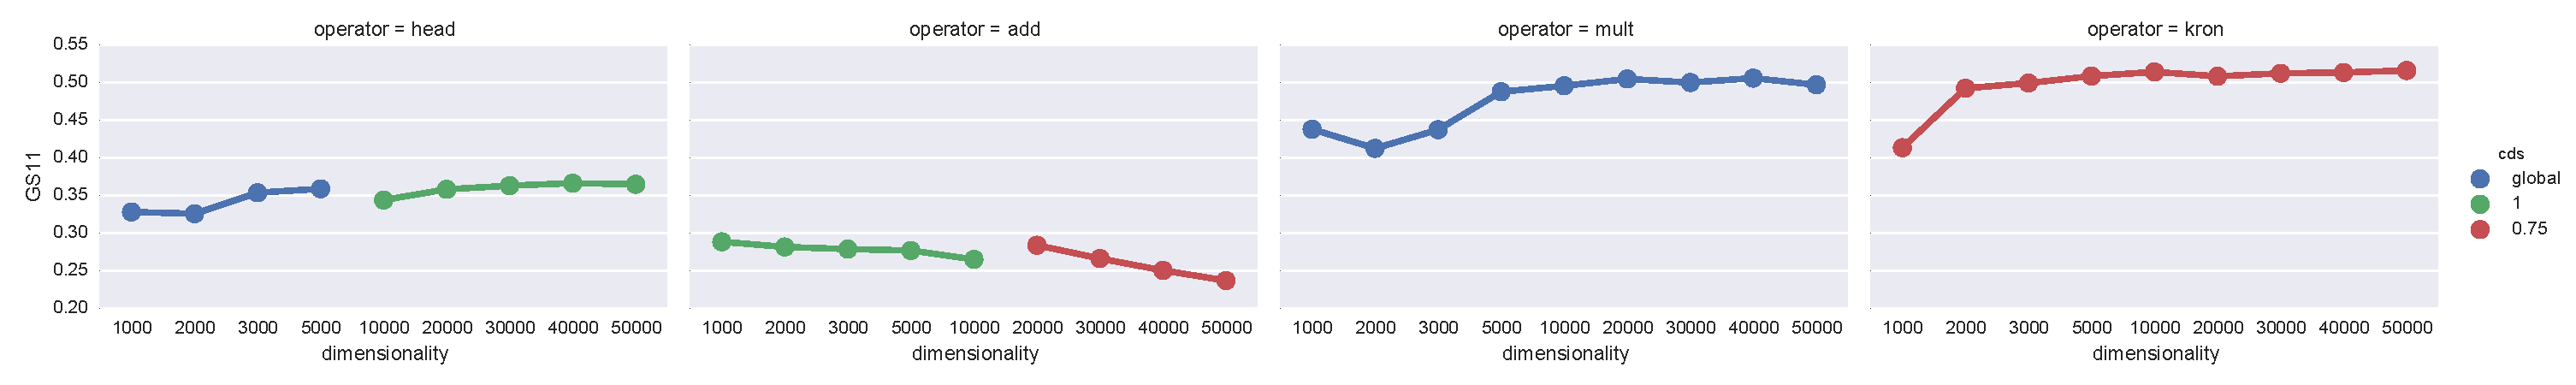
\includegraphics[width=\textwidth]{supplement/figures/GS11-heuristics-selection-cds}
    \caption{H. CDS.}
    \label{fig:}
  \end{subfigure}

  \begin{subfigure}[t]{0.7\textwidth}
    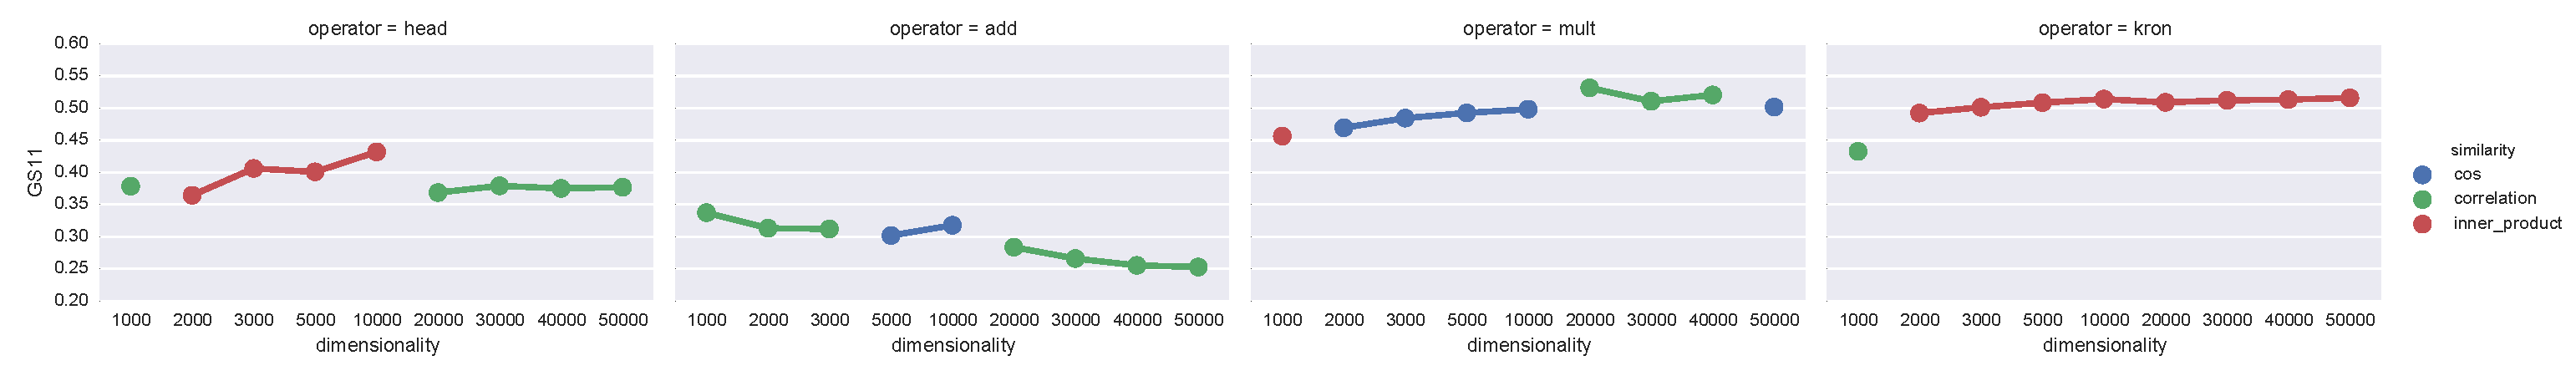
\includegraphics[width=\textwidth]{supplement/figures/GS11-max_-selection-similarity}
    \caption{Max. Sim.}
    \label{fig:}
  \end{subfigure}
  % \begin{subfigure}[t]{0.7\textwidth}
  %   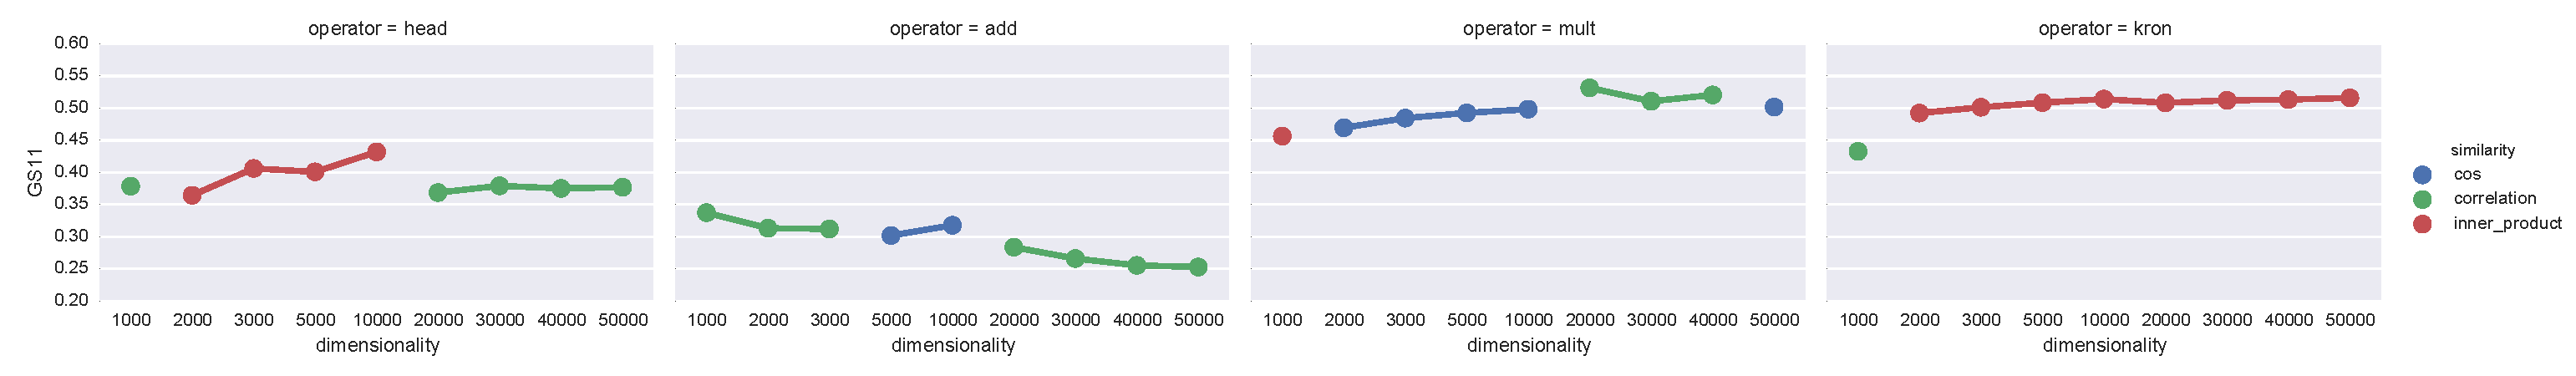
\includegraphics[width=\textwidth]{supplement/figures/GS11-cross_validation-selection-similarity}
  %   \caption{CV. Sim.}
  %   \label{fig:}
  % \end{subfigure}
  \begin{subfigure}[t]{0.7\textwidth}
    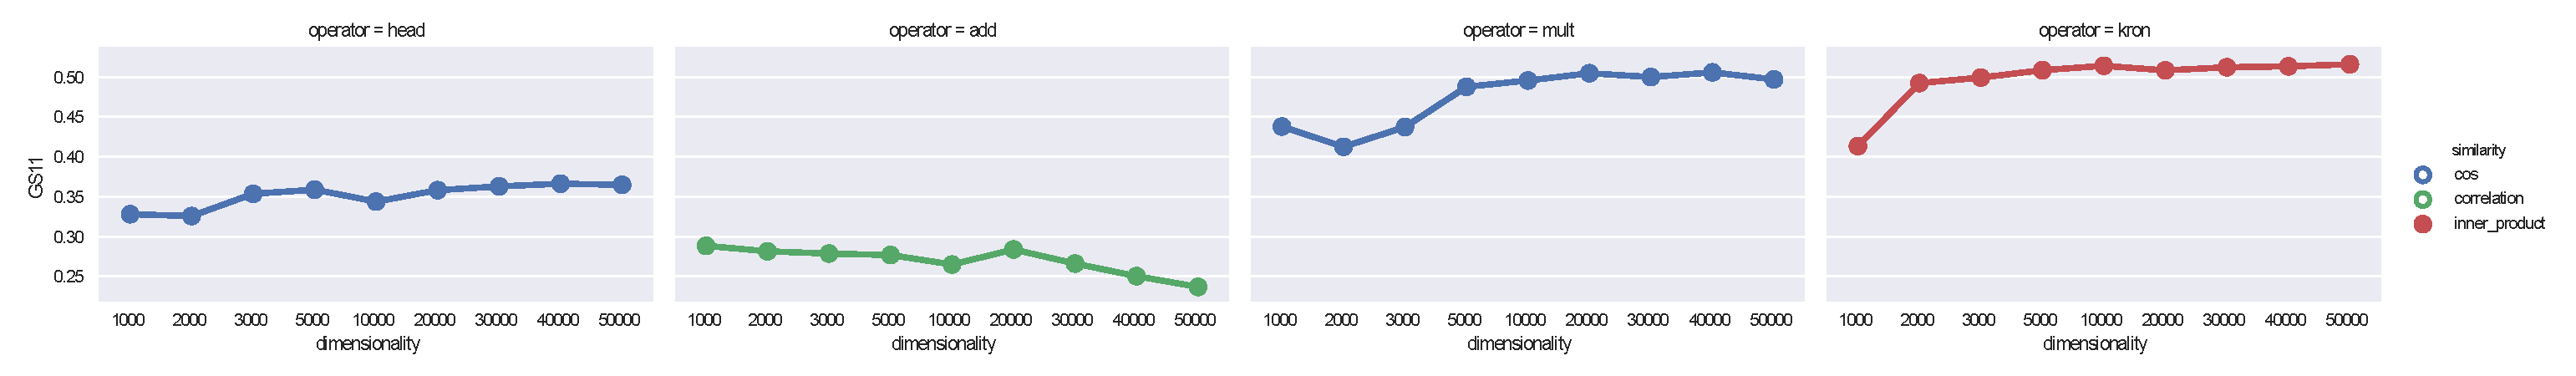
\includegraphics[width=\textwidth]{supplement/figures/GS11-heuristics-selection-similarity}
    \caption{H. Sim.}
    \label{fig:}
  \end{subfigure}

  \begin{subfigure}[t]{0.7\textwidth}
    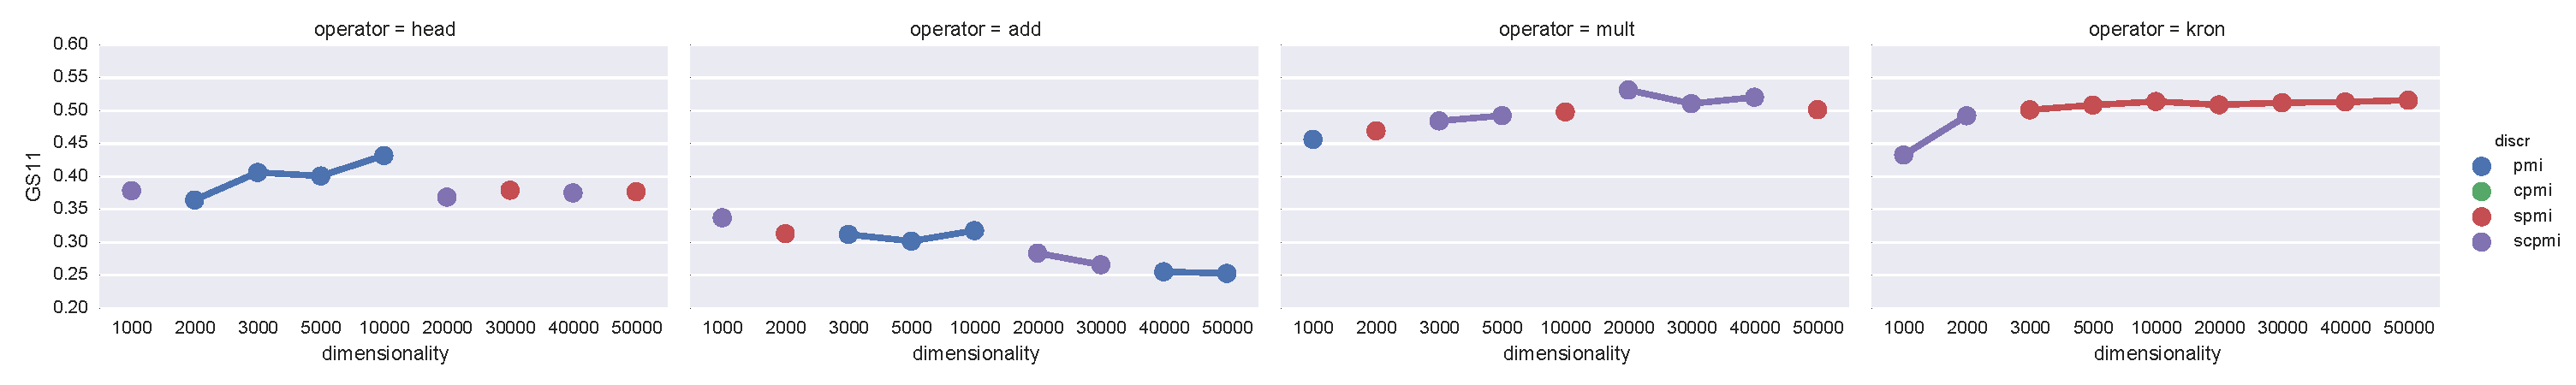
\includegraphics[width=\textwidth]{supplement/figures/GS11-max_-selection-discr}
    \caption{Max. Discr.}
    \label{fig:}
  \end{subfigure}
  % \begin{subfigure}[t]{0.7\textwidth}
  %   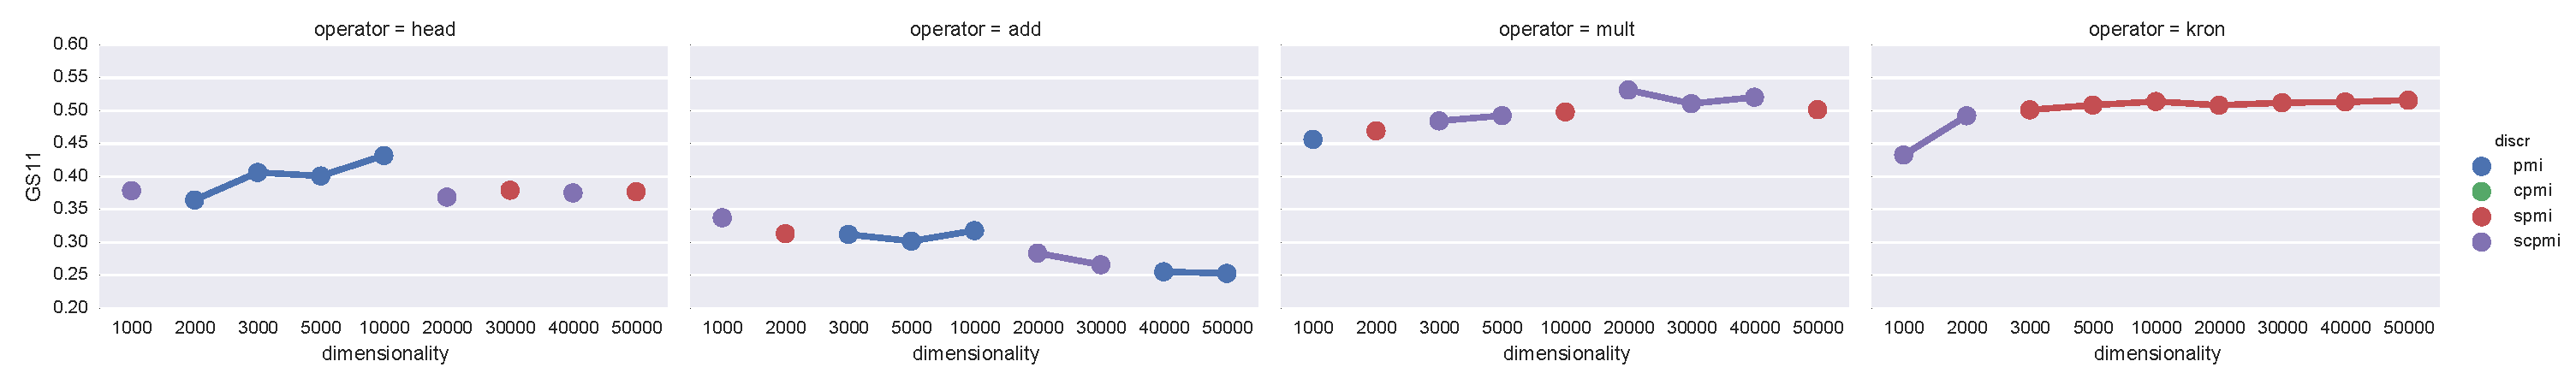
\includegraphics[width=\textwidth]{supplement/figures/GS11-cross_validation-selection-discr}
  %   \caption{CV. Discr.}
  %   \label{fig:}
  % \end{subfigure}
  \begin{subfigure}[t]{0.7\textwidth}
    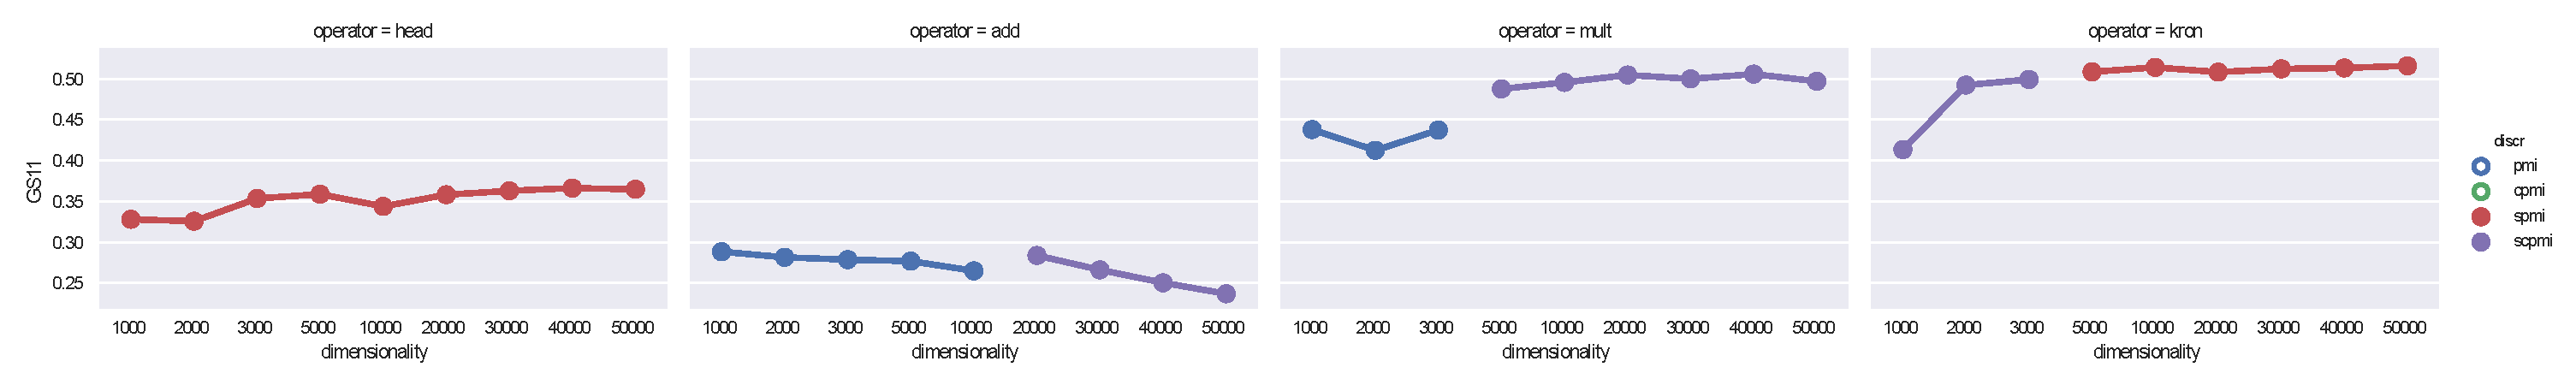
\includegraphics[width=\textwidth]{supplement/figures/GS11-heuristics-selection-discr}
    \caption{H. Discr.}
    \label{fig:}
  \end{subfigure}

  \caption{GS11 selection.}
  \label{fig:selection_gs11}
\end{figure}

\end{landscape}

\restoregeometry

% \clearpage
% \KOMAoptions{paper=A4,pagesize}
% \recalctypearea


% \subsection{GS12}
% \label{sec:gs12}

\subsection{Universal parameter selection for compositional datasets}
\label{sec:robust-param-comp-selecion}

\section{Universal parameter selection for lexical and compositional datasets}
\label{sec:universal-param-selection}



% \subsubsection{Tweaked IR evaluation}
% \label{sec:tweak-ir-eval}

% \todo[inline]{Discuss \cite{Milajevs:2015:IMN:2808194.2809448} and link to \ref{sec:phraserel}}

% \section{PhraseRel: relevance of sentences}
% \label{sec:sentential-relevance}

%%% Local Variables:
%%% mode: latex
%%% TeX-master: "thesis"
%%% End:
